\chapter{多色イメージングの効果の実証}      
MPPCと時定数の短いCe:YAP($\tau\sim25$ns)を用いることでパルス読み出しが可能となり個々のX線パルスを弁別することで、一度のX線照射で様々なエネルギー帯域での画像を取得することができる。複数のエネルギー帯域で画像を取得することにより、従来のエネルギー積分型のCTにおける問題点を解決できたり、新たな画像診断が可能となる。

\section{エネルギー分解能}
$^{57}$Coと$^{241}$Amを用いてMCA-8000Dで測定したスペクトルを\Fref{fig:57Co_241Am}に示す。また$^{57}$Coを照射した時のMPPCの信号波形を\Fref{fig:YAP_waveform}に示す。

\begin{figure}[H]
 \begin{center}
 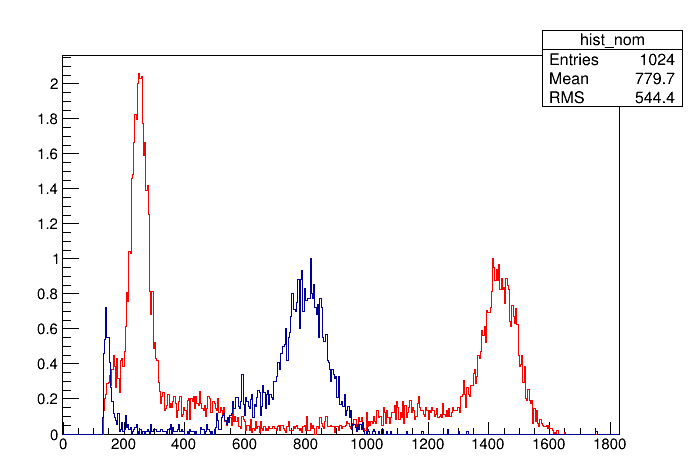
\includegraphics[bb=0.000000 0.000000 696.000000 474.000000,width=0.6\hsize]{image2/chapter5/241Am_57Co_Gain5_000_100ns.png} 
 \end{center}
 \caption{$^{57}$Coと$^{241}$Amのスペクトル}
 \label{fig:57Co_241Am}
\end{figure}

\begin{figure}[H]
 \begin{center}
 \includegraphics[bb=0.000000 0.000000 596.000000 536.000000,width=0.5\hsize]{image2/chapter5/57Co_YAP_Raw_wave.png} 
 \end{center}
 \caption{$^{57}$Coを照射したときのMPPCで読み出したCe:YAPの波形}
 \label{fig:YAP_waveform}
\end{figure}

エネルギー分解能は13.4\%(FWHM)@122keV、20.4\%(FWHM)@59.5keV であった。\Fref{fig:57Co_241Am}からチャンネルとエネルギーの関係を求めエネルギーキャリブレーションを行った。また、信号波形の時定数は50.3nsであった。


\section{多色イメージングの測定方法}

多色イメージングにおいては複数の閾値を設けるため\Fref{fig:read_circuit_pulse_multi}のようなエネルギー弁別回路となっている。\Fref{fig:read_circuit_pulse_multi}中の$V_{th4},V_{th3},V_{th2},V_{th1}$は\Fref{fig:spectrum_multi}のように設定したと仮定する。


\begin{figure}[H]
 \begin{center}
 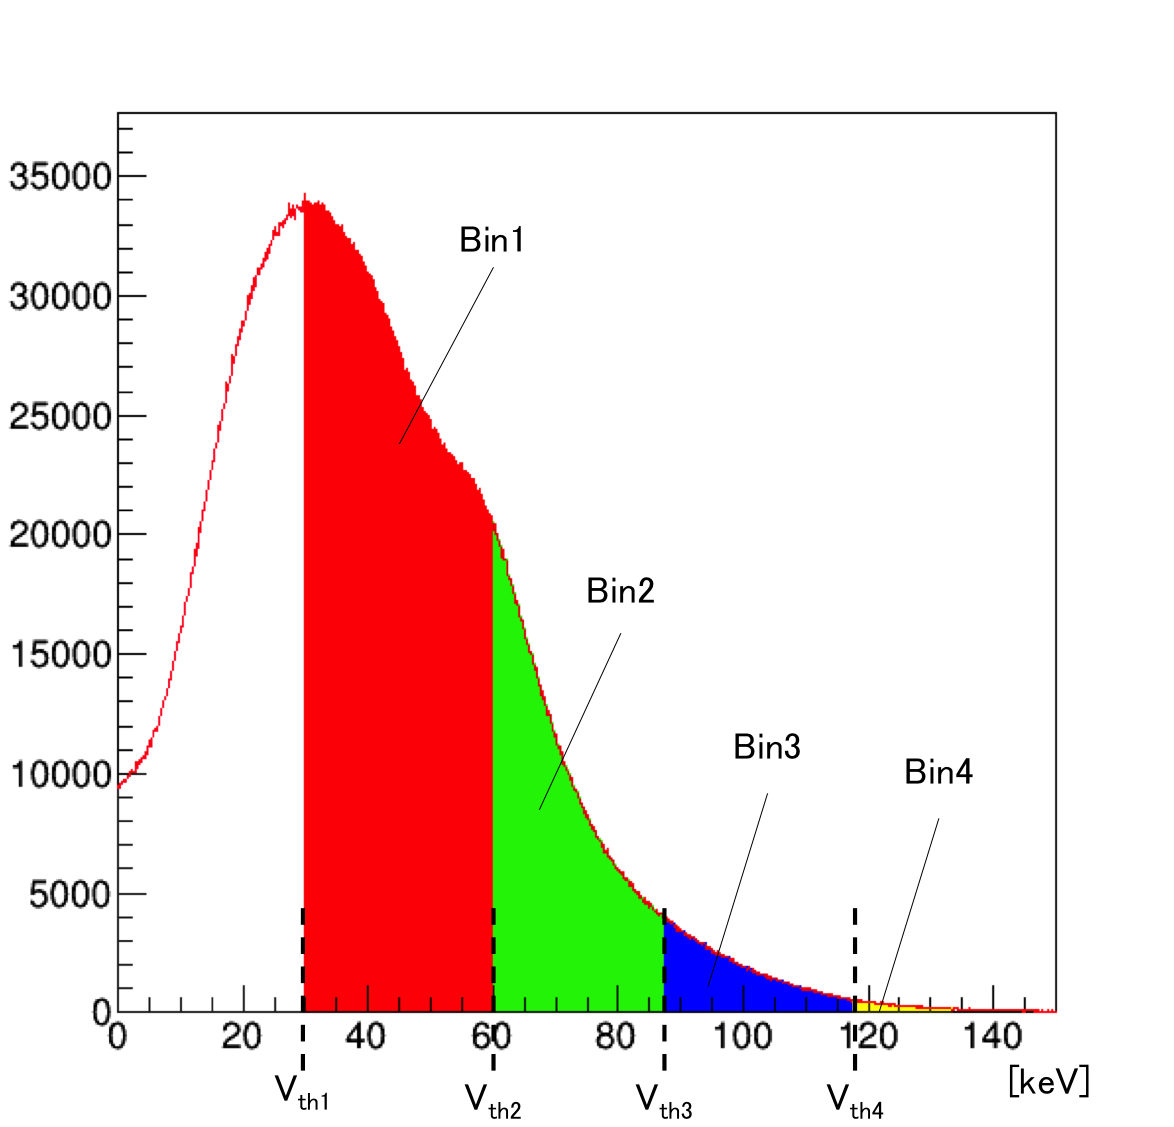
\includegraphics[bb=0.000000 0.000000 563.473420 540.915284,width=0.7\hsize]{image2/chapter5/spectrum_multi.png} 
 \end{center}
 \caption{多色イメージングの例}
 \label{fig:spectrum_multi}
\end{figure}


\begin{figure}[H]
 \begin{center}
 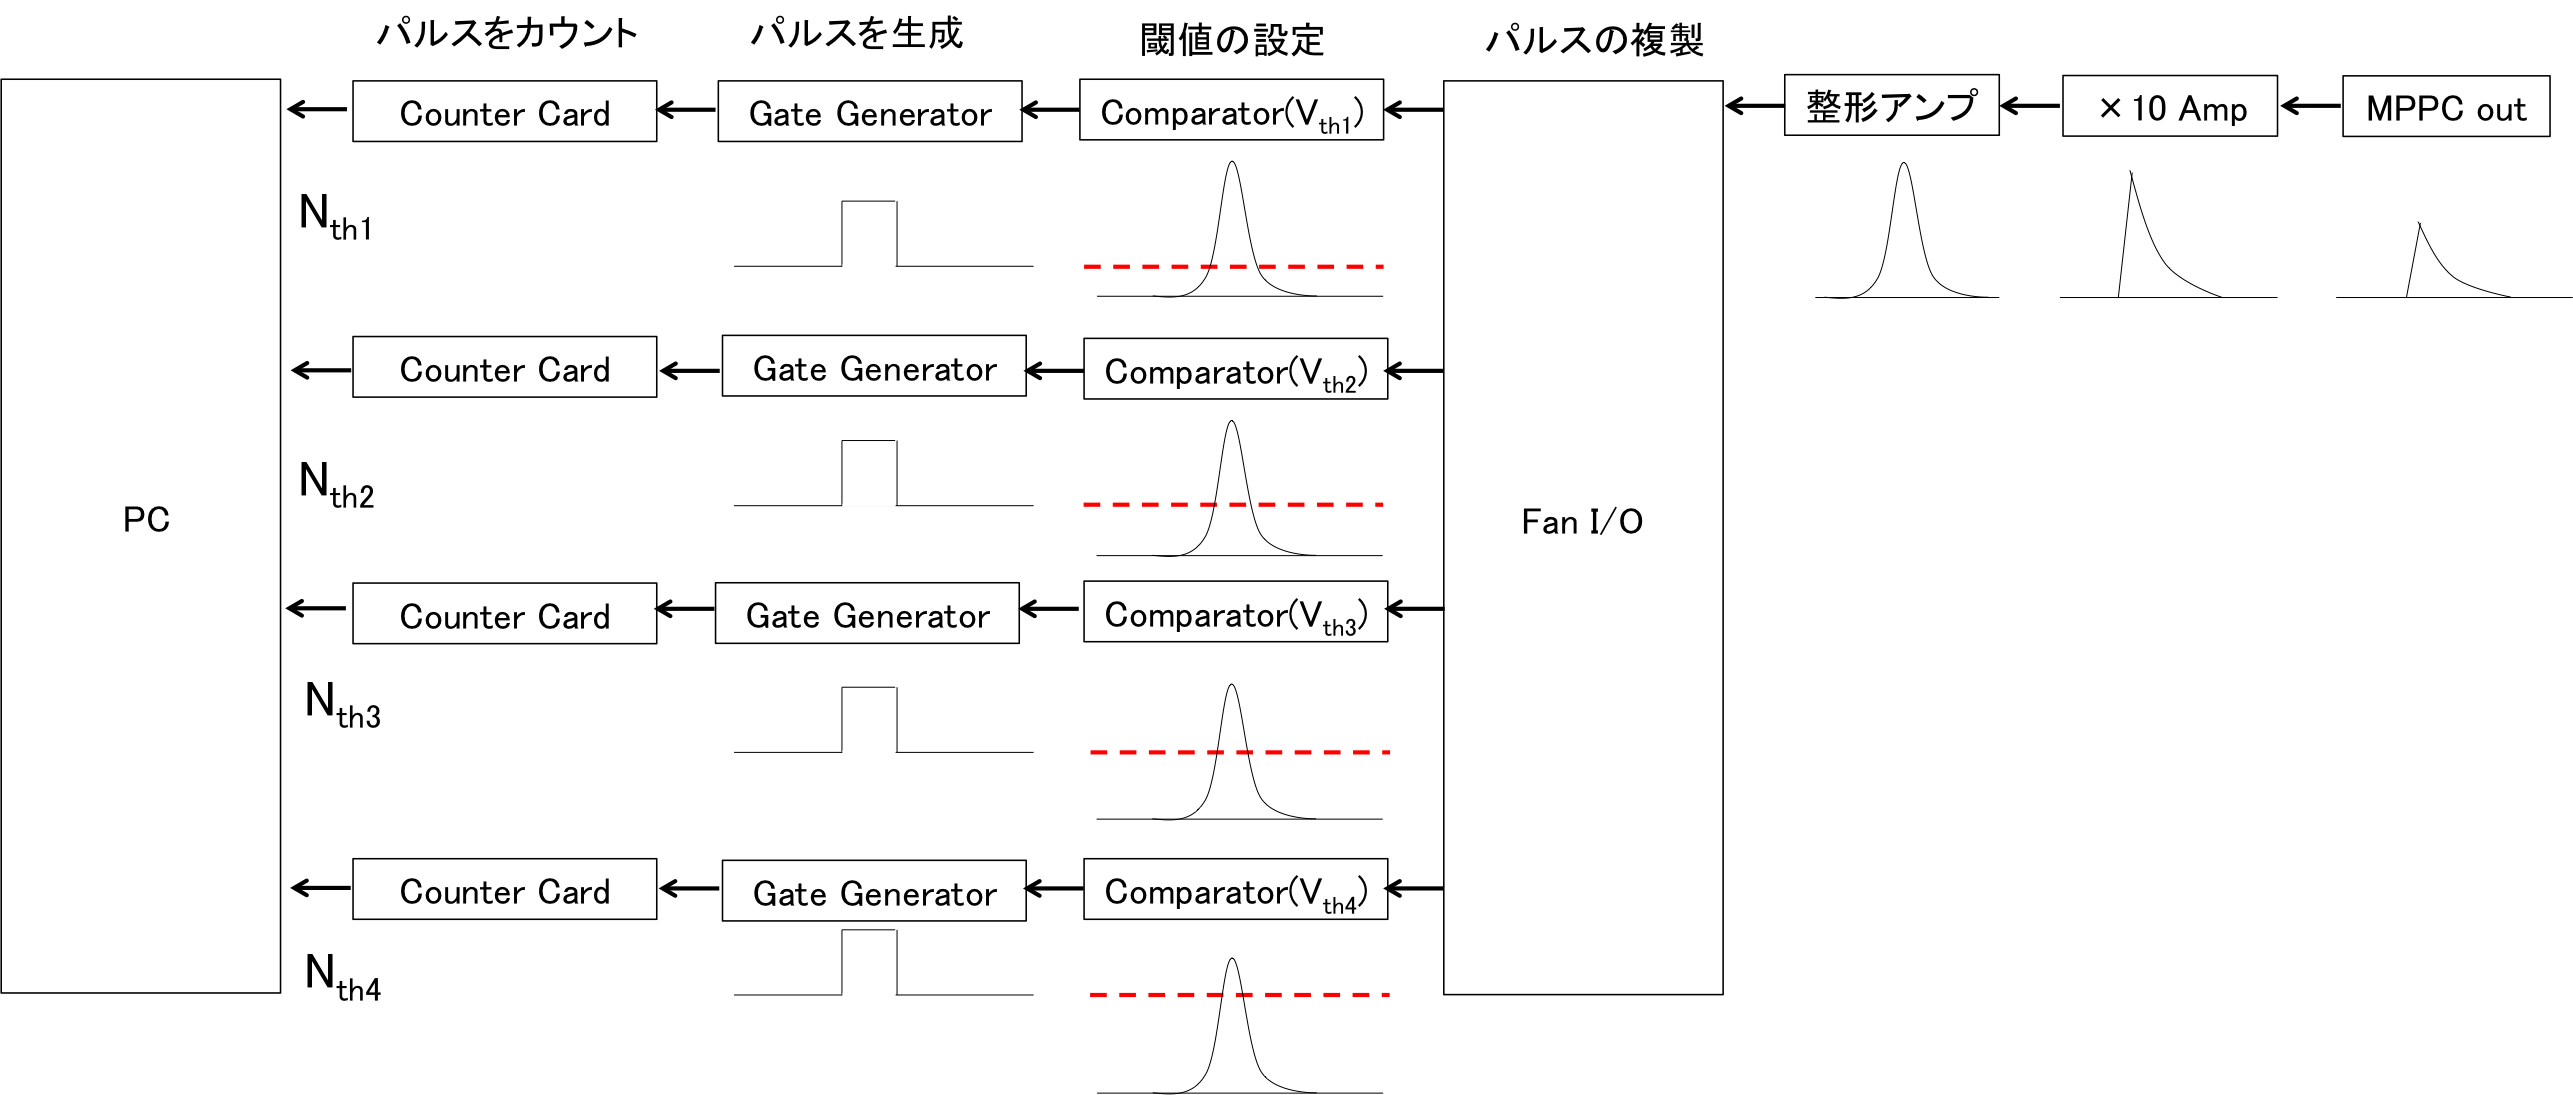
\includegraphics[bb=0.000000 0.000000 1234.937912 525.556554,width=1\hsize]{image2/chapter5/read_circuit_pulse_multi.png} 
 \end{center}
 \caption{多色イメージングのエネルギー弁別回路($V_{th4}>V_{th3}>V_{th2}>V_{th1}$)}
 \label{fig:read_circuit_pulse_multi}
\end{figure}

例えば閾値に$V_{th1}=30keV, V_{th2}=60keV, V_{th3}=90keV,$に設定したとき、それぞれの閾値を超える波高を持つ信号の例を\Fref{fig:120kV_0.1mA_multi_th}に示す。

\begin{figure}[H]
 \begin{center}
 \includegraphics[bb=0.000000 0.000000 696.000000 474.000000,width=0.7\hsize]{image2/chapter5/120kV_0.1mA_multi_th.png} 
 \end{center}
 \caption{$V_{th1}=30keV, V_{th2}=60keV, V_{th3}=90keV,$に設定したとき、それぞれの閾値を超える波高を持つ信号の例}
 \label{fig:120kV_0.1mA_multi_th}
\end{figure}

最大で4つの閾値を設けることが可能となる。\Fref{fig:spectrum_multi}示したようにBin1-Bin4まで複数のエネルギー帯域に置いて投影データを作成、それぞれのBinにおいて画像再構成を行う。それぞれのBinにおけるイベントは以下のように求めた。

\begin{align}
N_{Bin1}&=N_{th1}-N_{th2}\\
N_{Bin2}&=N_{th2}-N_{th3}\\
N_{Bin3}&=N_{th3}-N_{th4}\\
N_{Bin4}&=N_{th4}
\end{align}


本稿では多色イメージングの効果の検証として以下の項目の実証実験を行った。

\begin{itemize}
\item 低コントラスト分解能向上
\item ビームハードニング低減
\item 物質同定
\item K-edgeイメージング
\end{itemize}


\section{低コントラスト分解能向上}
?章で述べたようんX 線光子のエネルギーが低いほど光電吸収が支配的になるので線源弱係数の物質間での差が高エネルギーより大きくなるので,低エネルギー帯の反応イベントのみを用いてCT画像を取得することによりコントラストを強調することができる。
\Fref{fig:phantom1}に示したCT値が近い水とアルコールを用いて、アルコールと水のコントラスト強調実験を行った。水とアルコールの線減弱係数を\Fref{fig:water_alchol}に示す。

\begin{figure}[H]
 \begin{center}
 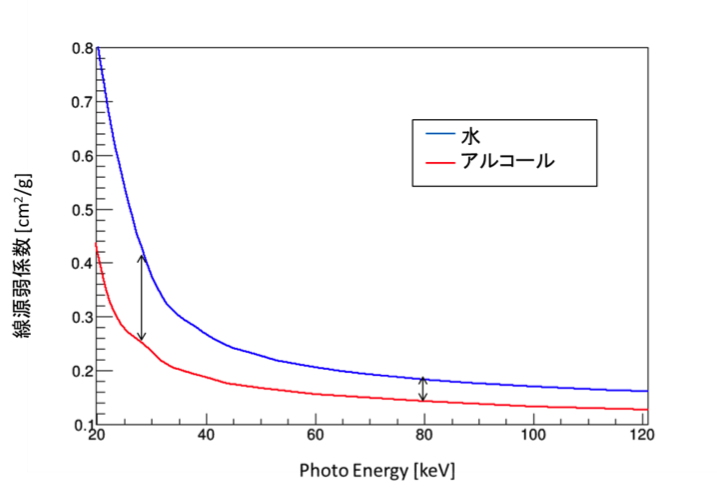
\includegraphics[bb=0.000000 0.000000 344.611512 237.580360,width=0.8\hsize]{image2/chapter5/water_alchol.png} 
 \end{center}
 \caption{水とアルコールの線減弱係数(NISTより作成)}
 \label{fig:water_alchol}
\end{figure}

閾値は20keV、40keV、60keV、80keVに設定し、管電圧120kV、管電流0.1mAにおける20-40keV、40-60keV、60-80keV、80-120keVのエネルギーバンドにおけるCT画像をそれぞれ取得し画像を比較した。


\subsection{実験結果}
まず。各閾値においてMCA-800Dを用いて測定したX線スペクトルを\Fref{fig:spectrum_low}に示す。
それぞれの閾値でスペクトルが明確に分離されていることがわかる。それぞれのエネルギーバンドで得られたCT画像を\Fref{fig:low_contrast_multi}に示す。

\begin{figure}[H]
 \begin{minipage}{0.52\hsize}
  \begin{center}
   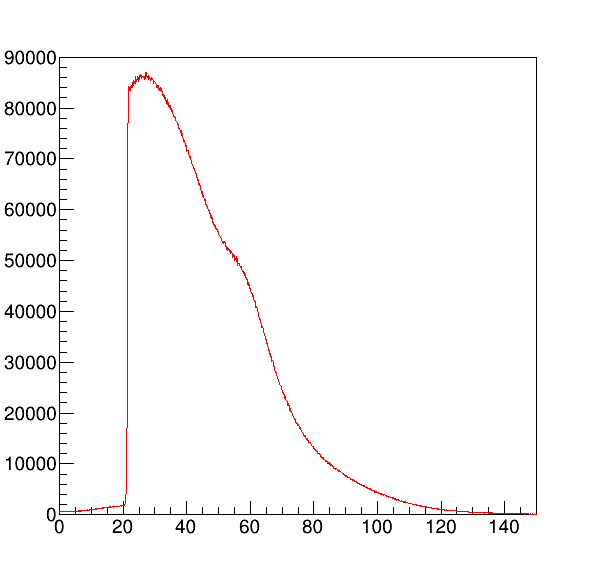
\includegraphics[bb=0.000000 0.000000 596.000000 574.000000,width=1.0\hsize]{image2/chapter5/120kV_0.1mA_20keV_100sec.png}
  \end{center}
\vspace{-1cm}
\caption*{(a)20keV}
 \end{minipage}
 \begin{minipage}{0.52\hsize}
  \begin{center}
    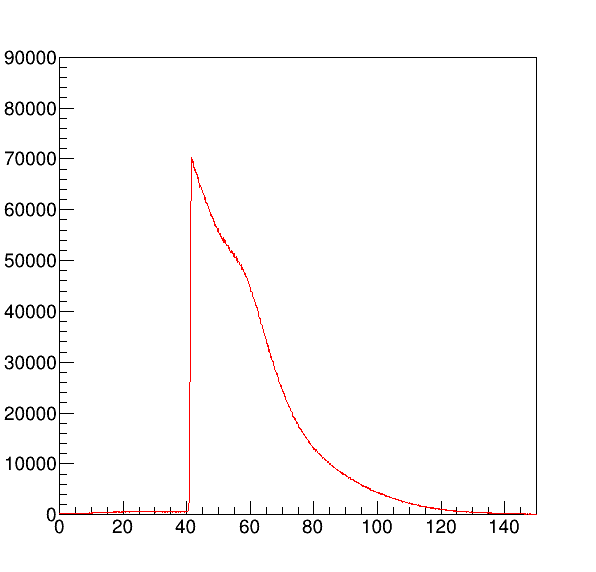
\includegraphics[bb=0.000000 0.000000 596.000000 574.000000,width=1.0\hsize]{image2/chapter5/120kV_0.1mA_40keV_100sec.png}
  \end{center}  
\vspace{-1cm}
\caption*{(b)40keV}
 \end{minipage}
   \begin{minipage}{0.5\hsize}
  \begin{center}
       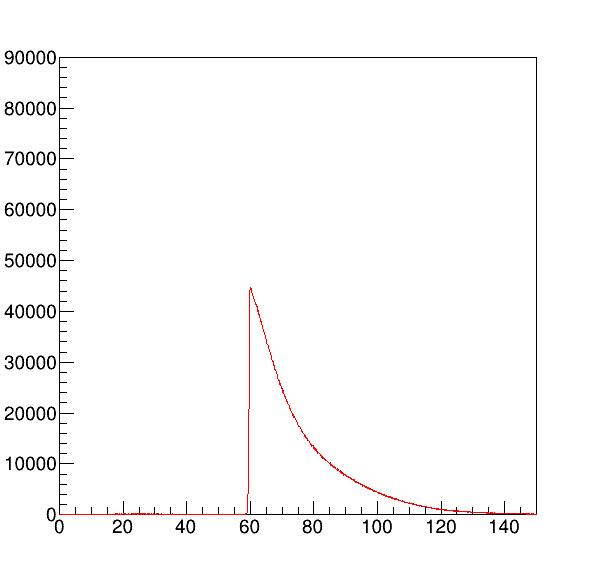
\includegraphics[bb=0.000000 0.000000 596.000000 574.000000,width=1.0\hsize]{image2/chapter5/120kV_0.1mA_60keV_100sec.png}
  \end{center}
  \vspace{-1cm}
\caption*{(c)60keV}
 \end{minipage}
 \begin{minipage}{0.5\hsize}
  \begin{center}
     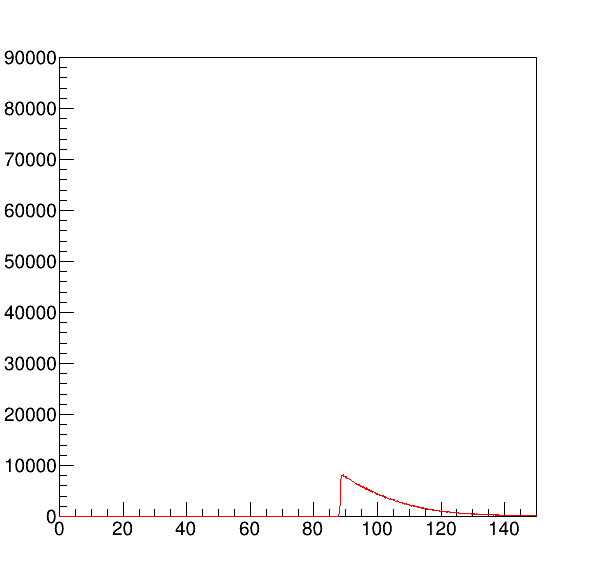
\includegraphics[bb=0.000000 0.000000 596.000000 574.000000,width=1.0\hsize]{image2/chapter5/120kV_0.1mA_90keV_100sec.png}
  \end{center}
 \vspace{-1cm}
\caption*{(d)80keV}
 \end{minipage}
 \begin{minipage}{0.5\hsize}
 \hspace{3cm} 
     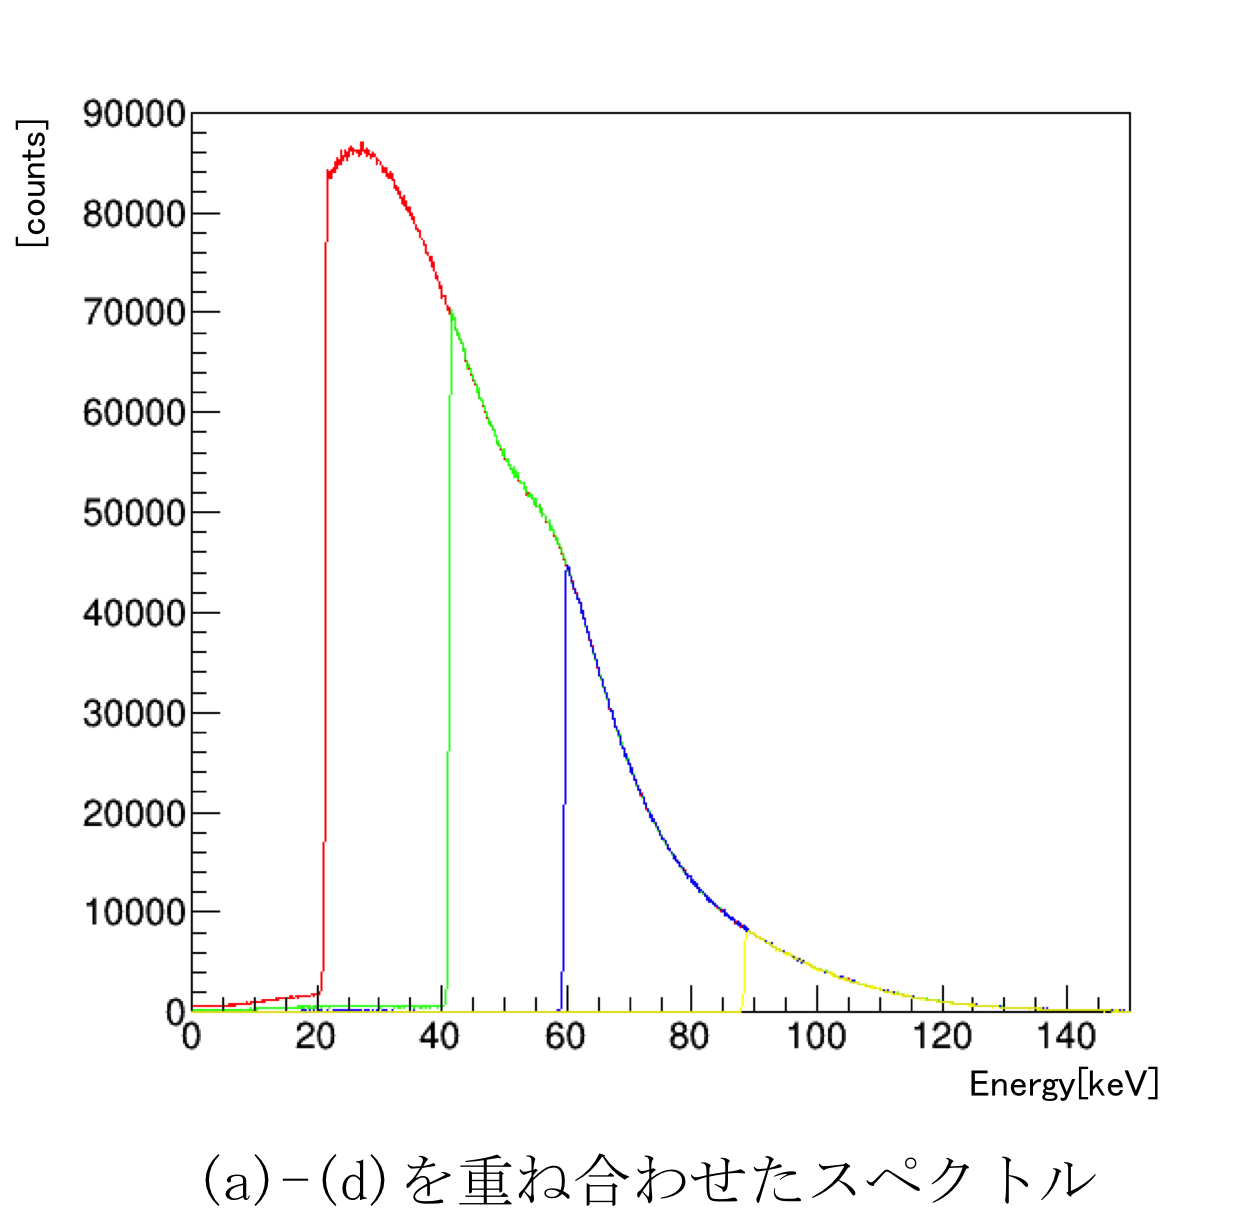
\includegraphics[bb=0.000000 0.000000 598.510523 586.031555,width=1.0\hsize]{image2/chapter5/120kV_0.1mA_V_100sec_multi.png}
 \vspace{-1cm}
 \end{minipage}
 \begin{center}
  \caption{各エネルギー閾値におけるX線エネルギースペクトル}
  \label{fig:spectrum_low}
  \end{center}
\end{figure}


\begin{figure}[H]
 \begin{minipage}{0.5\hsize}
  \begin{center}
   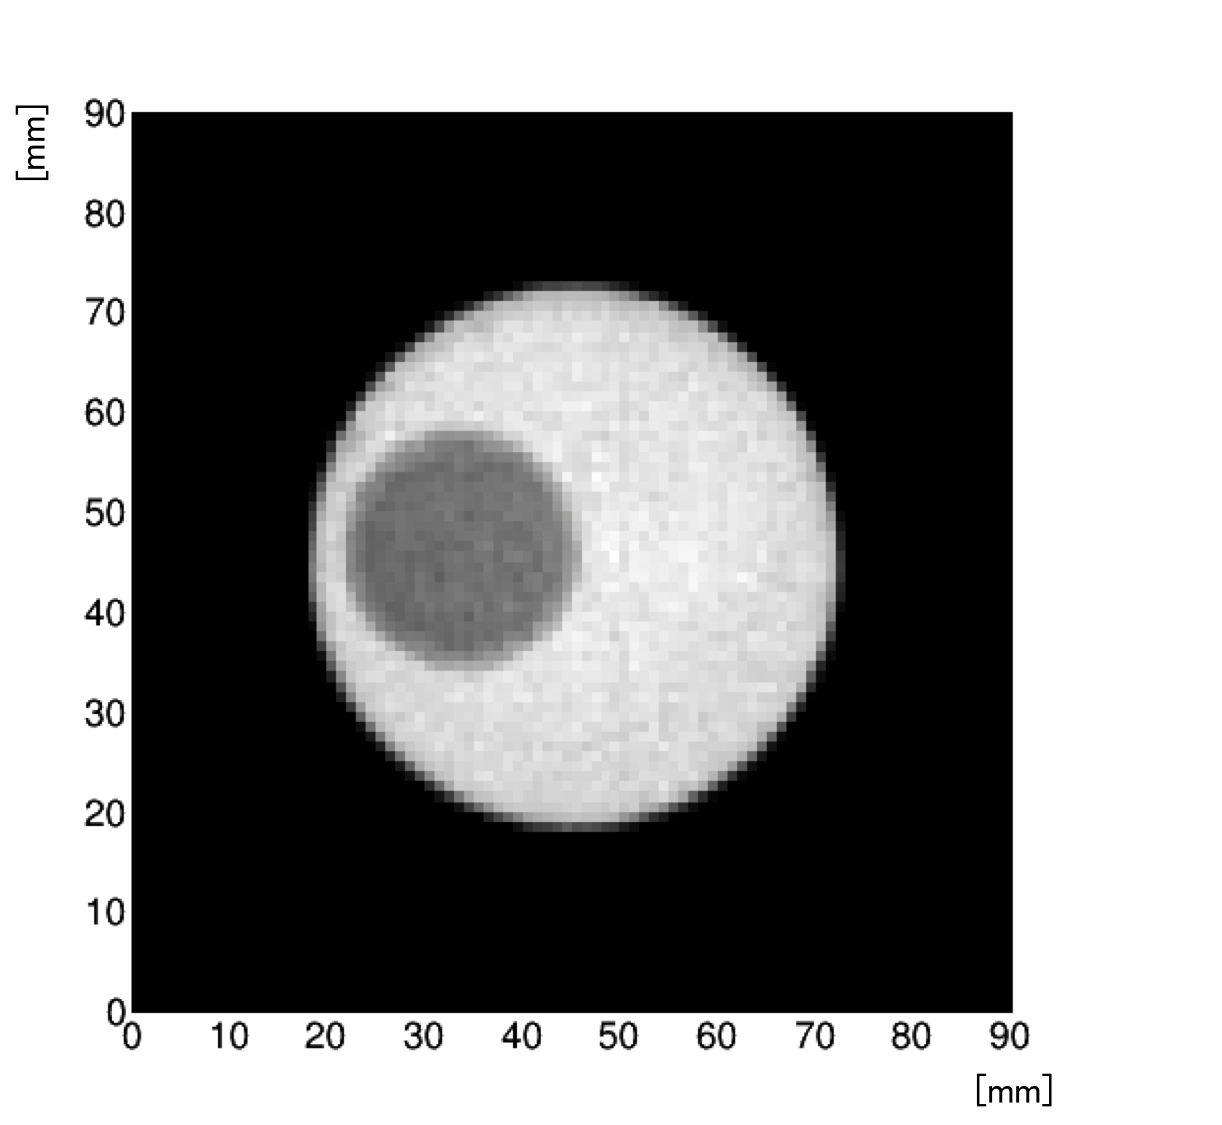
\includegraphics[bb=0.000000 0.000000 586.511515 539.955364,width=1.0\hsize]{image2/chapter5/low_contrast_20-40.png}
  \end{center}  
\vspace{-1cm}
\caption*{(a)20-40keV}
 \end{minipage}
 \begin{minipage}{0.5\hsize}
  \begin{center}
   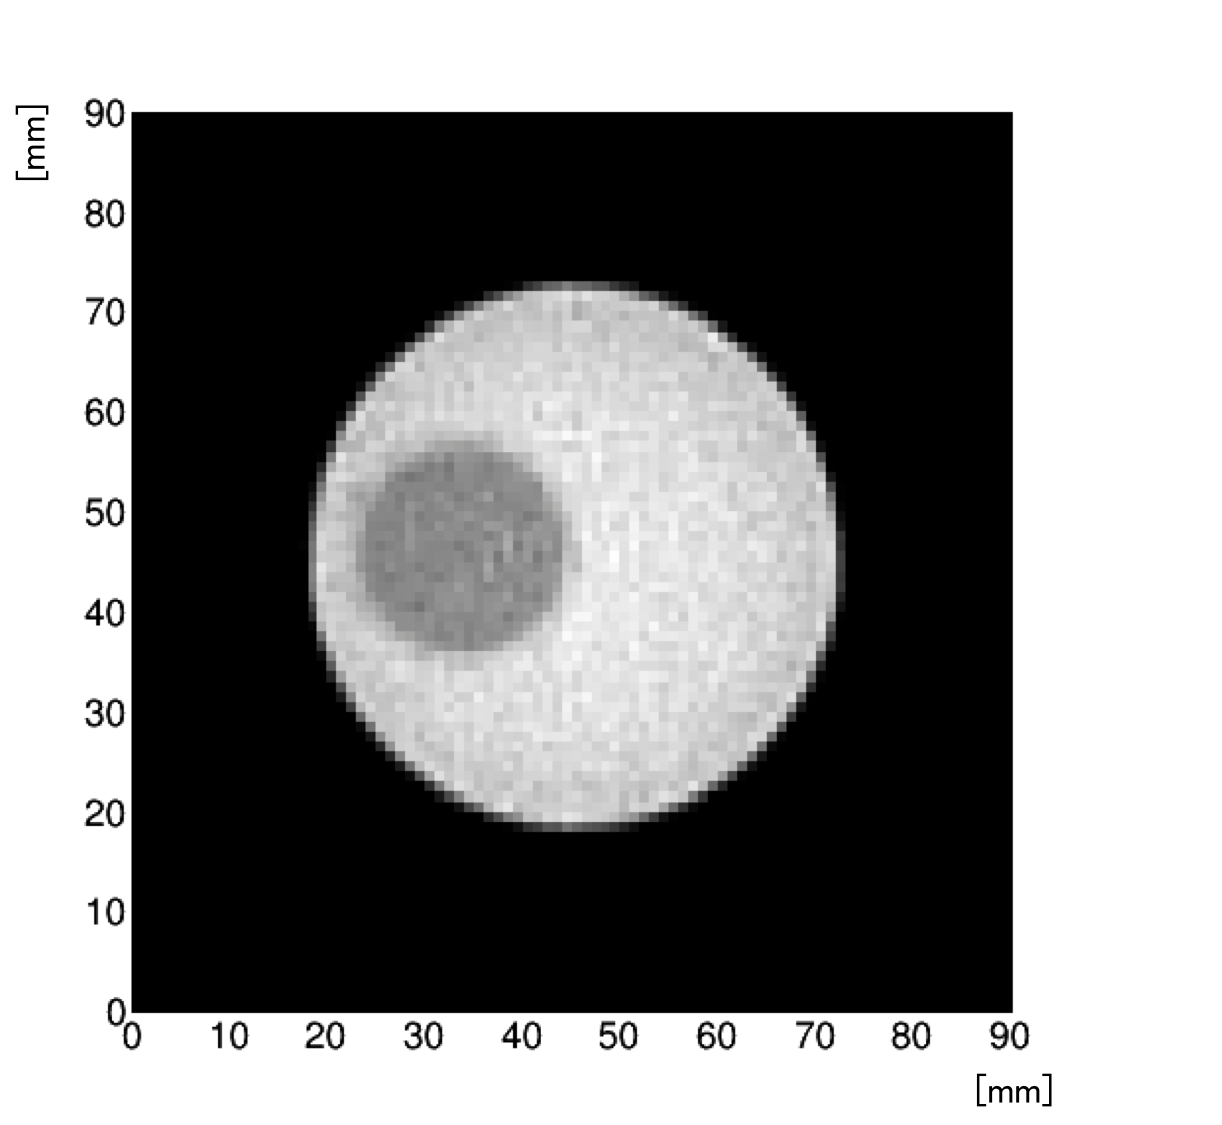
\includegraphics[bb=0.000000 0.000000 586.511515 539.955364,width=1.0\hsize]{image2/chapter5/low_contrast_40-60.png}
  \end{center}
\vspace{-1cm}
\caption*{(b)40-60keV}
 \end{minipage}
 \begin{minipage}{0.5\hsize}
  \begin{center}
   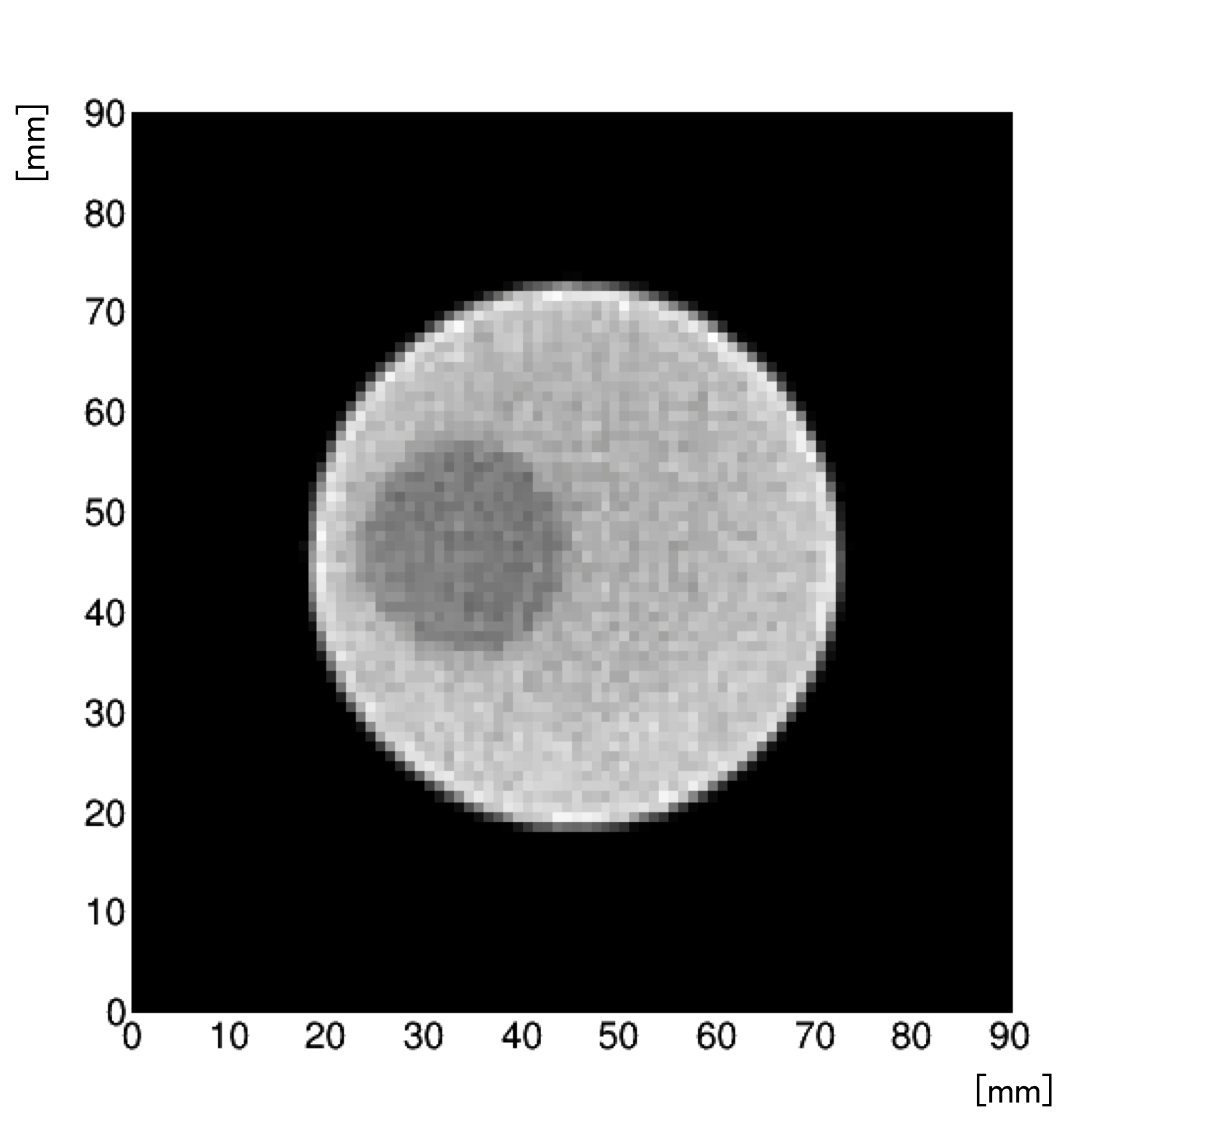
\includegraphics[bb=0.000000 0.000000 586.511515 539.955364,width=1.0\hsize]{image2/chapter5/low_contrast_60-90.png}
  \end{center}  
\vspace{-1cm}
\caption*{(c)60-80keV}
 \end{minipage}
 \begin{minipage}{0.5\hsize}
  \begin{center}
   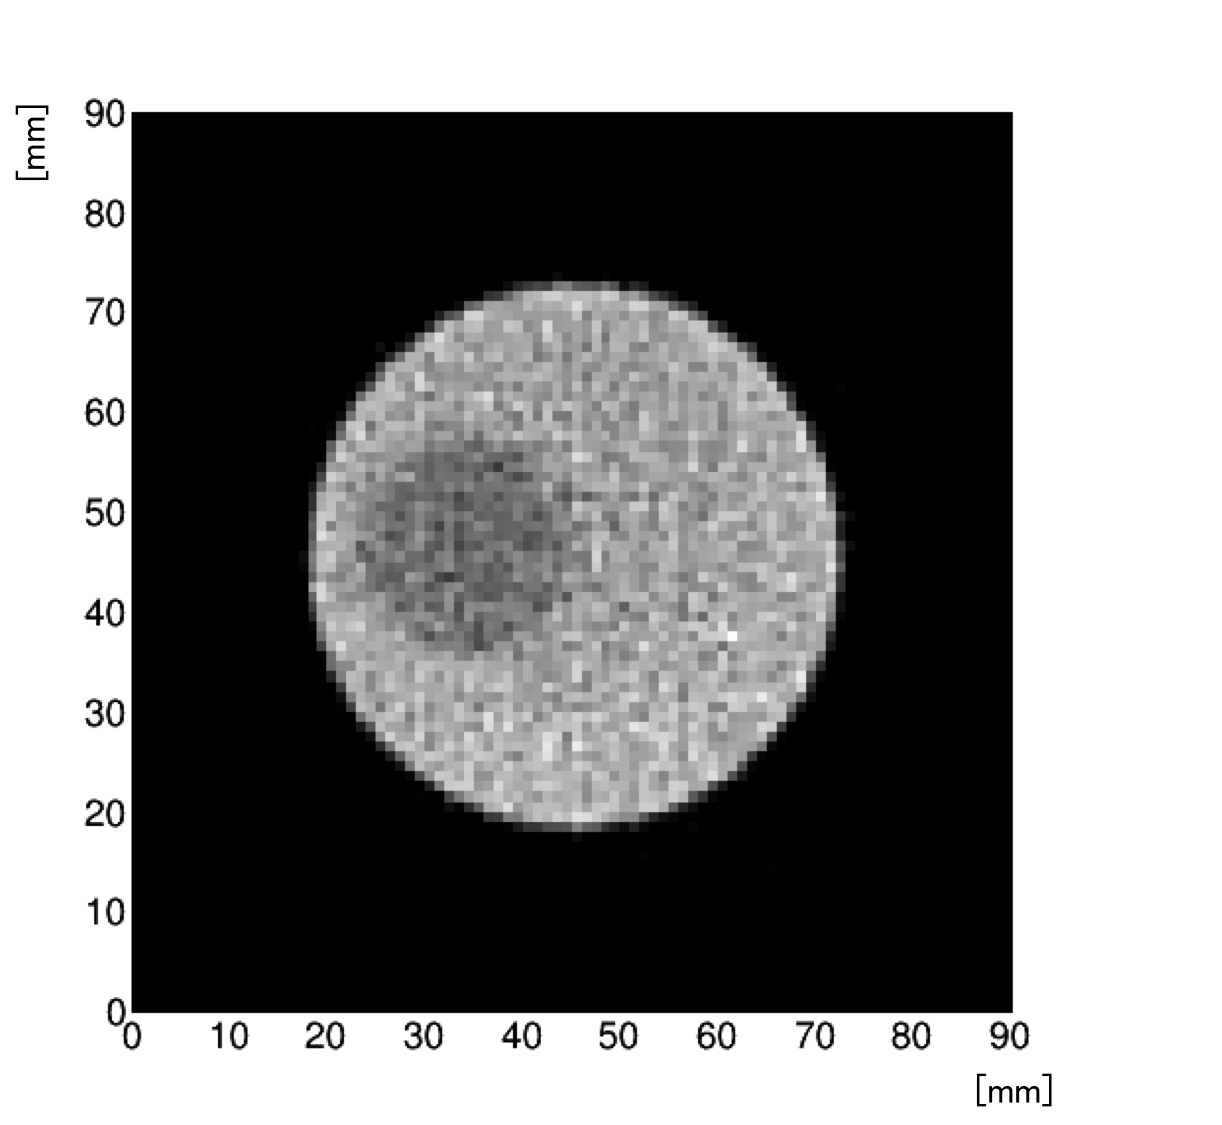
\includegraphics[bb=0.000000 0.000000 586.511515 539.955364,width=1.0\hsize]{image2/chapter5/low_contrast_90-120.png}
  \end{center}
\vspace{-1cm}
\caption*{(d)80-120keV}
 \end{minipage}
 \begin{minipage}{0.5\hsize}
  \begin{center}
   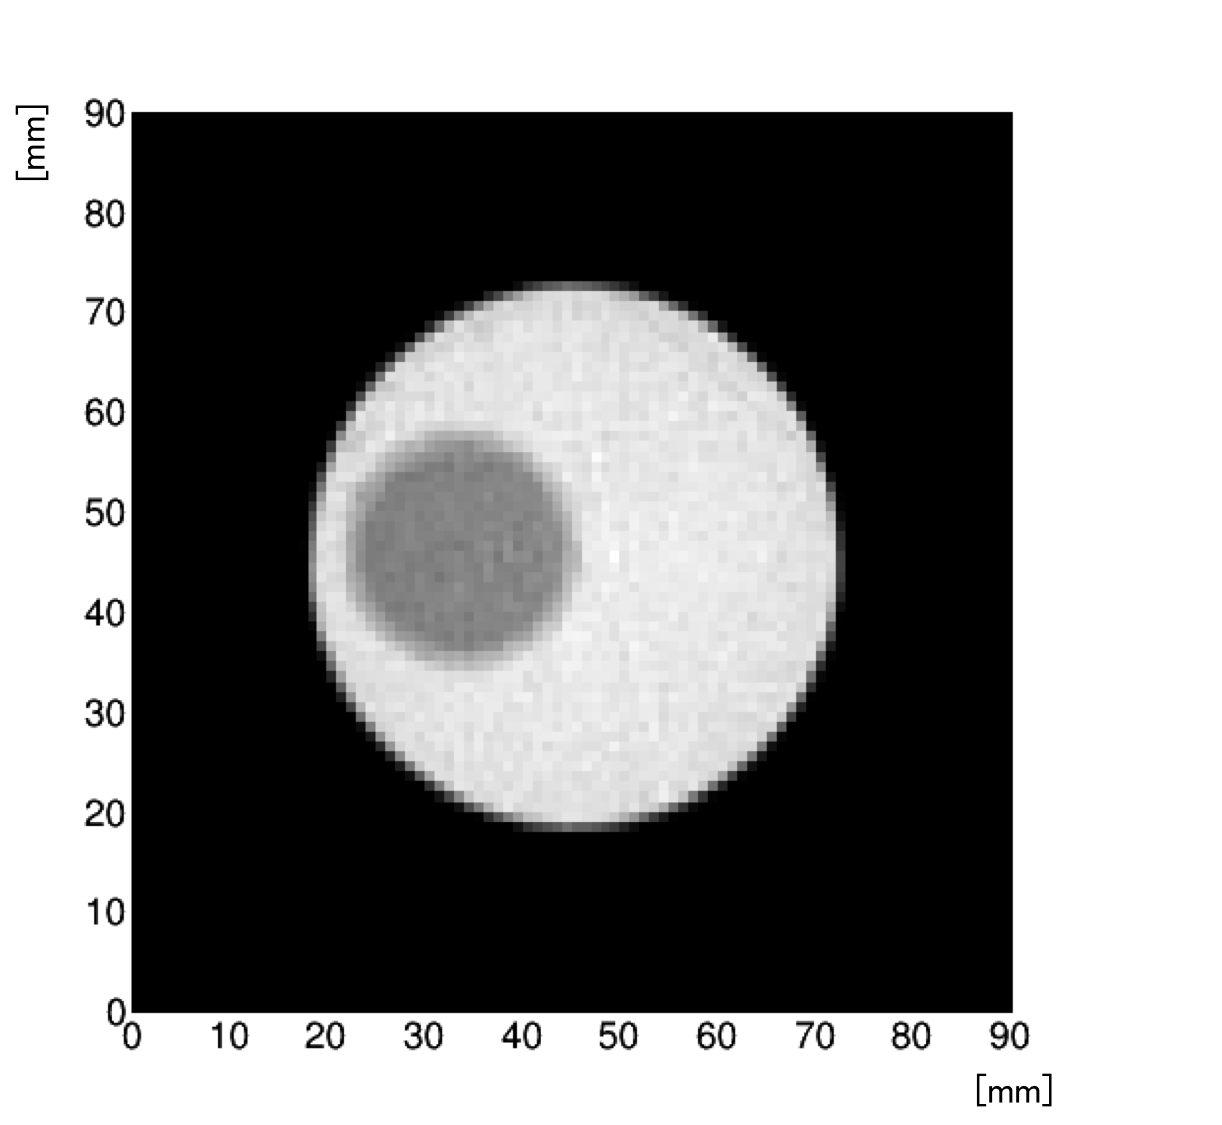
\includegraphics[bb=0.000000 0.000000 586.511515 539.955364,width=1.0\hsize]{image2/chapter5/low_contrast_20-120.png}
  \end{center}  
\vspace{-1cm}
\caption*{(e)全エネルギー(20-120keV)}
 \end{minipage}
 \begin{center}
  \caption{\Fref{fig:phantom1}の全エネルギーと各エネルギーバンドにおけるCT画像}
  \label{fig:low_contrast_multi}
  \end{center}
\end{figure}


\begin{figure}[H]
 \begin{center}
 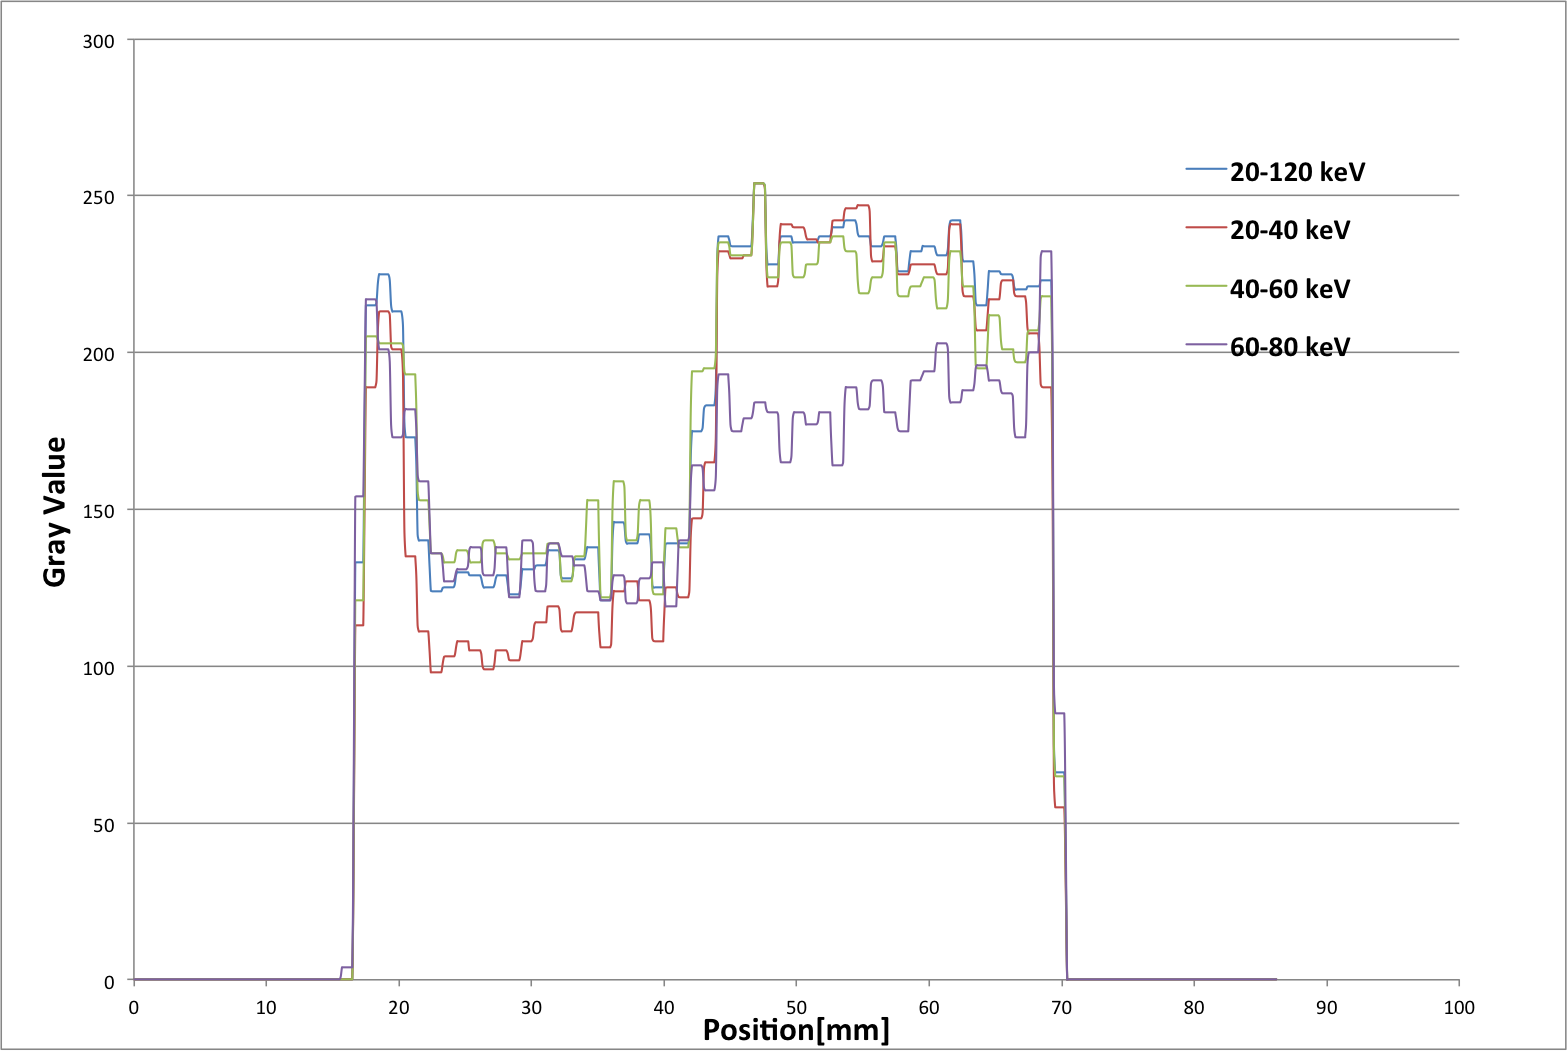
\includegraphics[bb=0.000000 0.000000 752.097827 504.438300,width=0.7\hsize]{image2/chapter5/Low_Con_slice.png} 
 \end{center}
 \caption{\Fref{fig:low_contrast_multi}の一次元プロファイル}
 \label{fig:Low_Con_slice}
\end{figure}


それぞれのエネルギーバンドで得られた画像につてコントラスト比($\mu_{alcohol}/\mu_{water}$)とCNRを算出した結果を\Tref{tab:low_contrast}に示す。
% Table generated by Excel2LaTeX from sheet 'Sheet1'
\begin{table}[H]
  \centering
    \begin{tabular}{cccccc}
    \toprule
    \multirow{2}[2]{*}{} & 全エネルギー & \multirow{2}[2]{*}{20-40 keV} & \multirow{2}[2]{*}{40-60 keV} & \multirow{2}[2]{*}{60-80keV} & \multirow{2}[2]{*}{80-120keV} \\
          & (20-120keV) &       &       &       &  \\
    \midrule
    コントラスト比 & \multirow{2}[1]{*}{0.63} & \multirow{2}[1]{*}{0.56} & \multirow{2}[1]{*}{0.67} & \multirow{2}[1]{*}{0.73} & \multirow{2}[1]{*}{0.73} \\
    ($\mu_{alcohol}/\mu_{water}$) &       &       &       &       &  \\
    CNR   & 21.3  & 19.0    & 10.2  & 5.74  & 2.35 \\
    \bottomrule
    \end{tabular}%
      \caption{各エネルギーバンドでのCT画像のコントラスト比とCNR}
  \label{tab:low_contrast}%
\end{table}%


\Fref{fig:low_contrast_multi}を見ると、全エネルギーのときと比べると、20-40keVの画像の方が最もアルコールが暗くなっていることが目視でわかる。また一次元プロファイルを見ても20-40keVの画像のアルコールの部分が他のエネルギーバンドの画像に比べて顕著にそのCT値が低くなっていることがわかる。\Tref{tab:low_contrast}を見るとコントラスト比は全エネルギーでは0.63、低エネルギーのみを用いた時は0.56となり、コントラスト比を見てもアルコールと水のコントラストが向上していることがわかり、底エネルギー側を用いた多色イメージングの効果が実証できた。CNRが全エネルギーに比べて、各エネルギーバンドでの値が小さくなっているのは統計数が減少したことで画像ノイズ$\sigma$が増加したためである。

\section{ビームハードニング低減}
混合エネルギーのX線が物質を透過する際、低エネルギーのX線が多く吸収され、X線の実効エネルギーが高くなる現象をビームハードニング(BH)とよぶ。これにより、高原子番号の被写体をCT撮影した際にアーチファクト生じる。ここではを\Fref{fig:Al_Al}のような2本のアルミニウム柱を水中におき、管電圧150kV、管電流1.0mAでAPDとMPPCパルスモードでCT撮影を行った。30keV,60keV,90keVと120keVに閾値を設定し、全エネルギーのCT画像と高エネルギーバンド(90-120keV)のCT画像をそれぞれ取得し画像比較を行った。

\begin{figure}[H]
 \begin{center}
 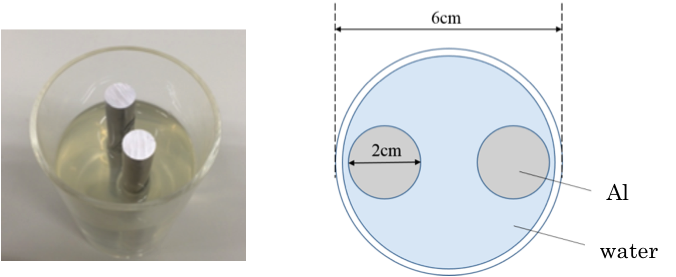
\includegraphics[bb=0.000000 0.000000 324.453179 132.949010,width=0.7\hsize]{image2/chapter5/Al_Al.png} 
 \end{center}
 \caption{測定ファントム}
 \label{fig:Al_Al}
\end{figure}

\subsection{実験結果}

\begin{figure}[H]
 \begin{minipage}{0.5\hsize}
  \begin{center}
   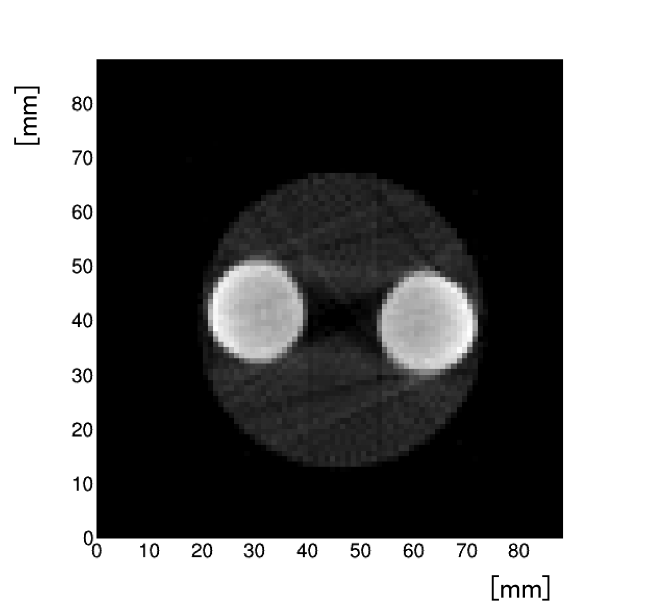
\includegraphics[bb=0.000000 0.000000 314.853972 293.735718,width=1.0\hsize]{image2/chapter5/BH_30-60.png}
  \end{center}  
\vspace{-1cm}
\caption*{(a)30-60keV}
 \end{minipage}
 \begin{minipage}{0.5\hsize}
  \begin{center}
   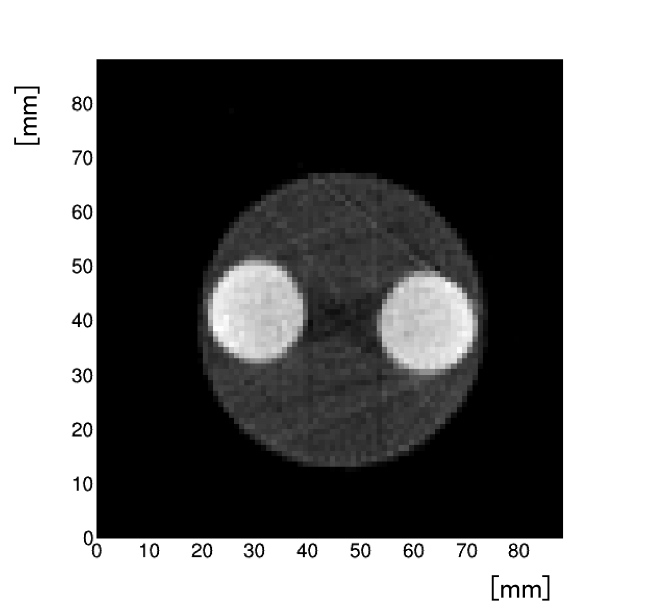
\includegraphics[bb=0.000000 0.000000 314.853972 293.735718,width=1.0\hsize]{image2/chapter5/BH_60-90.png}
  \end{center}
\vspace{-1cm}
\caption*{(b)60-90keV}
 \end{minipage}
 \begin{minipage}{0.5\hsize}
  \begin{center}
   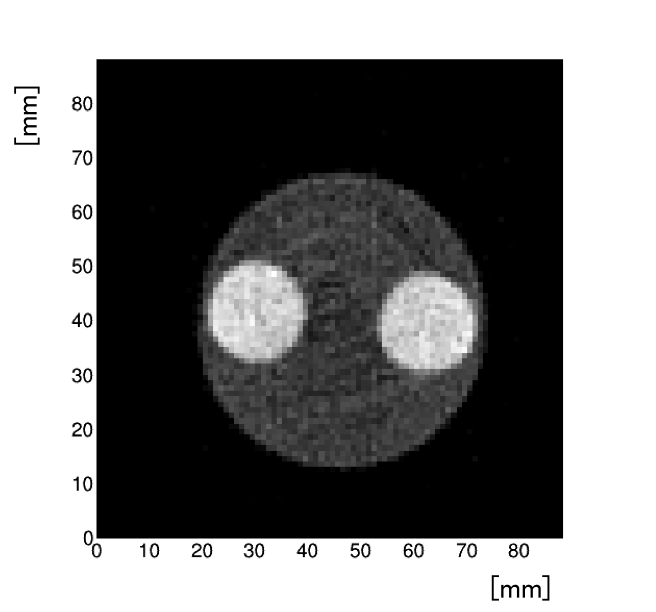
\includegraphics[bb=0.000000 0.000000 314.853972 293.735718,width=1.0\hsize]{image2/chapter5/BH_90-120.png}
  \end{center}  
\vspace{-1cm}
\caption*{(c)90-120keV}
 \end{minipage}
 \begin{minipage}{0.5\hsize}
  \begin{center}
   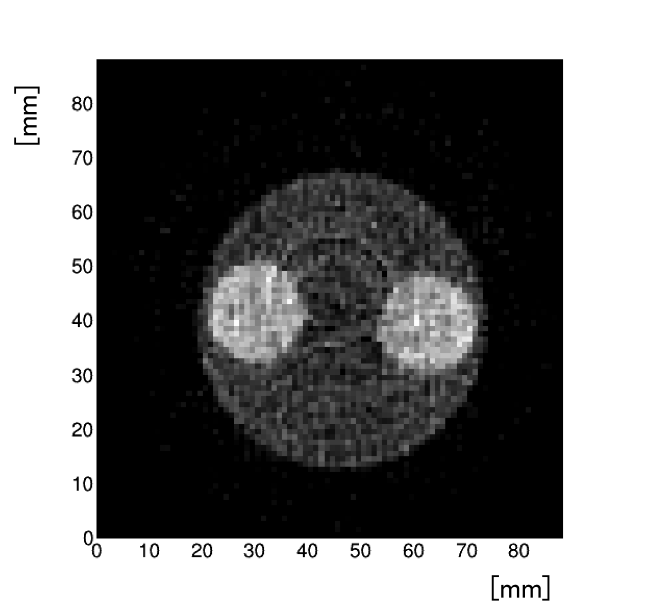
\includegraphics[bb=0.000000 0.000000 314.853972 293.735718,width=1.0\hsize]{image2/chapter5/BH_120-150.png}
  \end{center}
\vspace{-1cm}
\caption*{(d)120-150keV}
 \end{minipage}
 \begin{minipage}{0.5\hsize}
  \begin{center}
   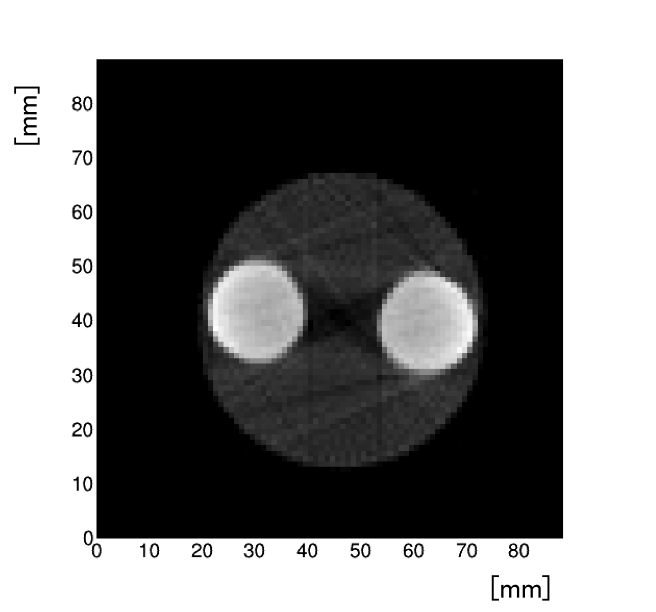
\includegraphics[bb=0.000000 0.000000 314.853972 293.735718,width=1.0\hsize]{image2/chapter5/BH_all.png}
  \end{center}  
\vspace{-1cm}
\caption*{(e)全エネルギー(20-150keV)}
 \end{minipage}
  \begin{minipage}{0.5\hsize}
  \begin{center}
   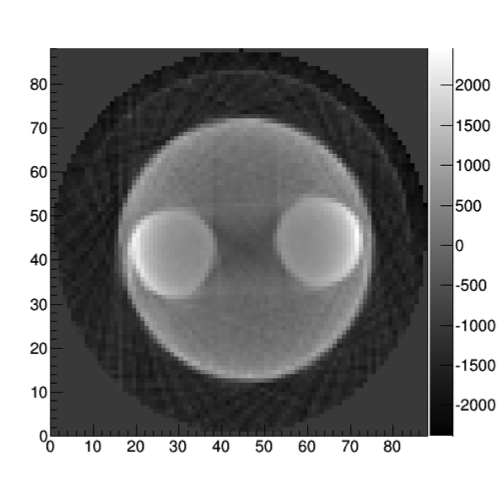
\includegraphics[bb=0.000000 0.000000 241.900003 232.780757,width=1.0\hsize]{image2/chapter5/BH_APD.png}
  \end{center}  
\vspace{-1cm}
\caption*{(f)全エネルギー(APD)}
 \end{minipage}
 \begin{center}
  \caption{\Fref{fig:Al_Al}の全エネルギーと各エネルギーバンドにおけるCT画像}
  \label{fig:BH_multi}
  \end{center}
\end{figure}

\begin{figure}[H]
 \begin{center}
 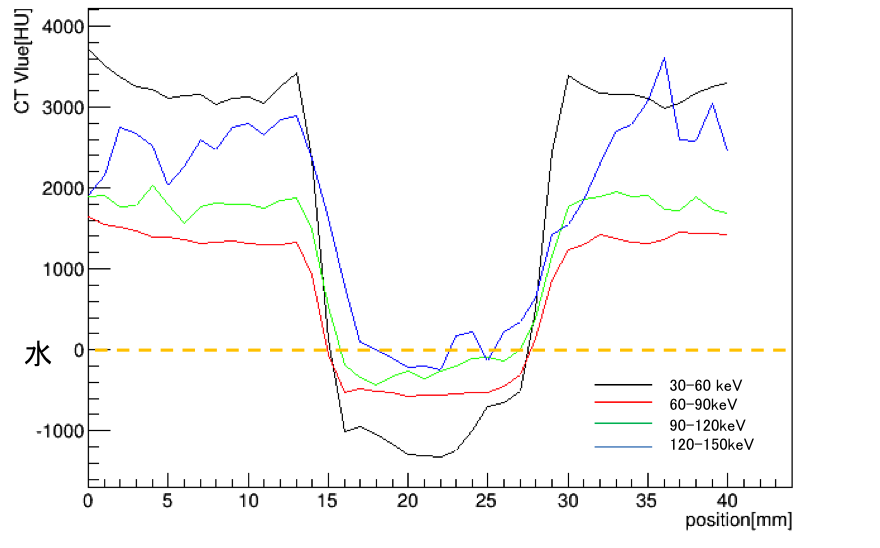
\includegraphics[bb=0.000000 0.000000 422.365084 263.018257,width=0.6\hsize]{image2/chapter5/BH_slice.png} 
 \end{center}
 \caption{\Fref{fig:BH_multi}の一次元プロファイル}
 \label{fig:BH_slice}
\end{figure}

全エネルギー情報を用いて取得した画像では、減弱係数の大きいAl円柱の間で画像が暗くなるアーチファクトが生じていることがわかる。それに対し、高エネルギーバンドのCT画像ではそれが見られず、\Fref{fig:BH_slice}を見ると高エネルギーバンドのCT画像ほどCT値が水のCT値である0に近く、ビームハードニングアーチファクトの低減に成功した。
120-150keVのCT画像のノイズが多いのは統計量が十分でなかったためである。
?でも述べたがビームハードニングアーチファクトは頭部や肩・骨盤内など骨に囲まれた部位に現れ出血や梗塞などの診断を困難にしていたが、高エネルギーバンドを用いた多色イメージングがビームハードニングアーチファクトを低減しその診断に有用であることが実証された。


\section{物質同定}
従来のエネルギー積分型のCT では,線源弱係数は物質が異なっても密度によっては同一になる場合があり,パラメータは一つのCT 値のみであったため正確な物質の弁別をすることができなかった。しかし,スペクトラルCT ではいくつかのエネルギー帯においてCT 値を取得することができるため,パラメータが複数になることで正確な材質の弁別が可能となる。本実験では、水とアルコールとアクリルの原子番号を求める実験を行った。ディスクリの位置を20keV、40kreV、60keVに設定し20-40keVのエネルギー帯と40-60keVのエネルギー帯でそれぞれCT撮影を管電圧120kV、管電流0.2mAで行った。20-40keVの平均エネルギーを25keV、40-60keVの平均エネルギーを45keVとして、CT画像のそれぞれのピクセルにおいて$k=\mu(25keV)/\mu(45keV)$を求めた。$k$の原子番号依存性はNISTから算出することができ、それを以下のように$f(z)$と定義する。

\begin{align}
f(Z)=\frac{\mu(Z,25keV)}{\mu(Z,45keV)}
\end{align}

NISTから求めた$k(Z)$の曲線を
\begin{align}
f(Z)=\frac{p_1+q_1Z+r_1Z^2}{p_2+q_2Z+r_2Z^2}
\end{align}

という関数でフィットしたっ結果を\Fref{fig:k_Z}に示す。

\begin{figure}[H]
 \begin{center}
 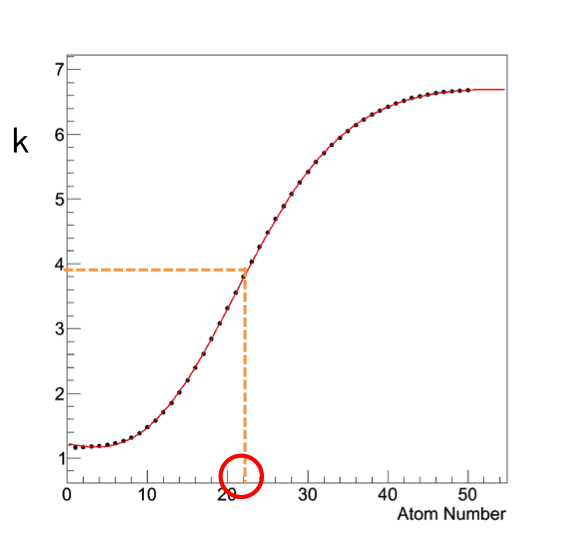
\includegraphics[bb=0.000000 0.000000 270.217662 258.218654,width=0.5\hsize]{image2/chapter5/k-Z.png} 
 \end{center}
 \caption{f(Z)の原子番号依存性(NISTより算出)}
 \label{fig:k_Z}
\end{figure}

それぞれのピクセルにおいて求めた$k$を用いて、$Z=f^{-1}(k)$を求めることでCT画像中の原審番号を同定することができる。
実効原子番号は\footnotetext{実効原子番号$Z_{\rm eff}$とは化合物や混合物において,単体における原子番号のどれくらいに相当するかを示す平均的な原子番号である。}は構成元素$Z_i$の電子数が全体に占める割合を$f_i$として$N$個の元素から構成されているとすると

\begin{align}
Z_{\rm eff}=\displaystyle\sum_{i=1}^{N}\sqrt[2.94]{f_i(Z_i)^{2.94}}
\end{align}

と求められる。これを用いて水、アルコール、PMMAの実効原子番号を求めた。

\subsection{実験結果}

\begin{figure}[H]
 \begin{minipage}{0.5\hsize}
  \begin{center}
   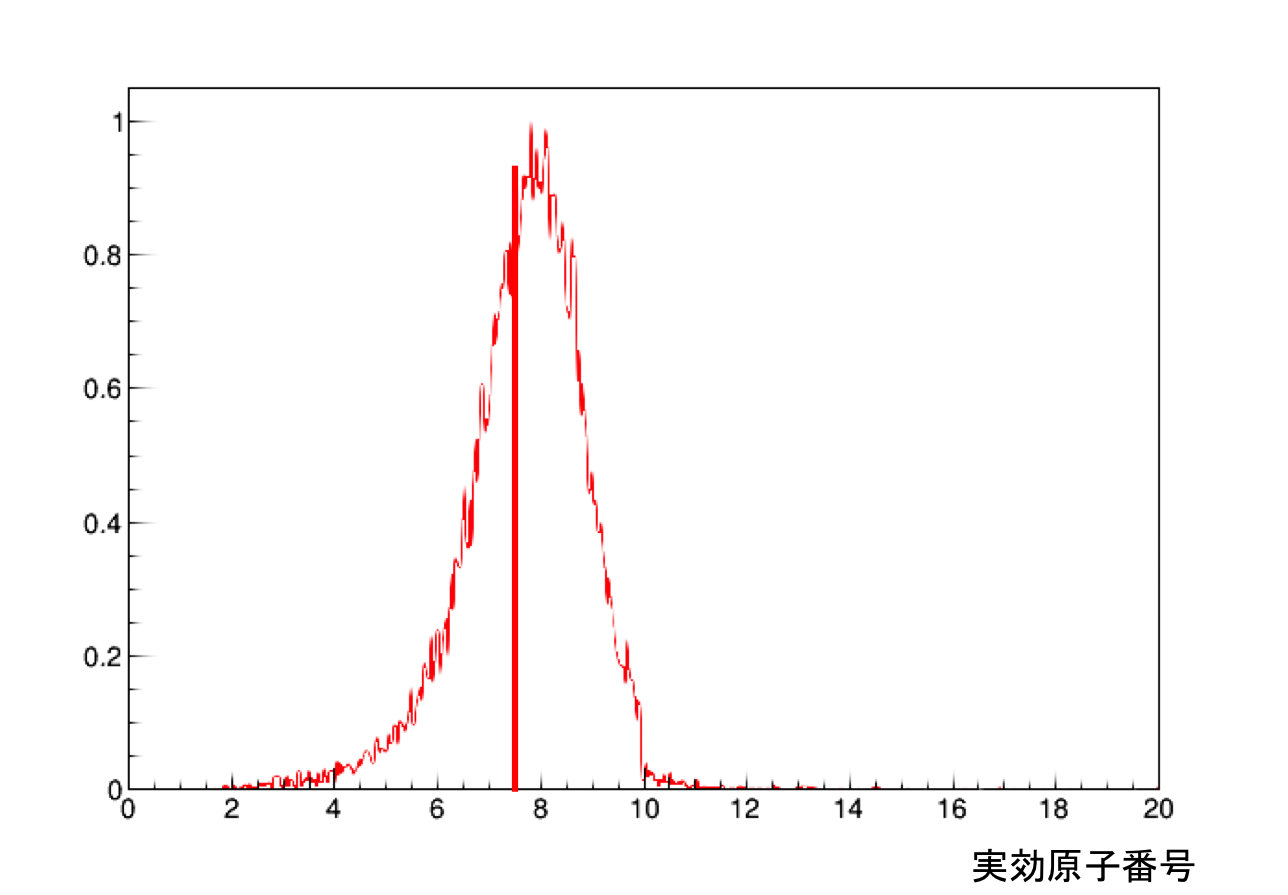
\includegraphics[bb=0.000000 0.000000 618.188896 429.564489,width=1.0\hsize]{image2/chapter5/Z_water.png}
  \end{center}  
\vspace{-1cm}
\caption*{水}
 \end{minipage}
 \begin{minipage}{0.5\hsize}
  \begin{center}
   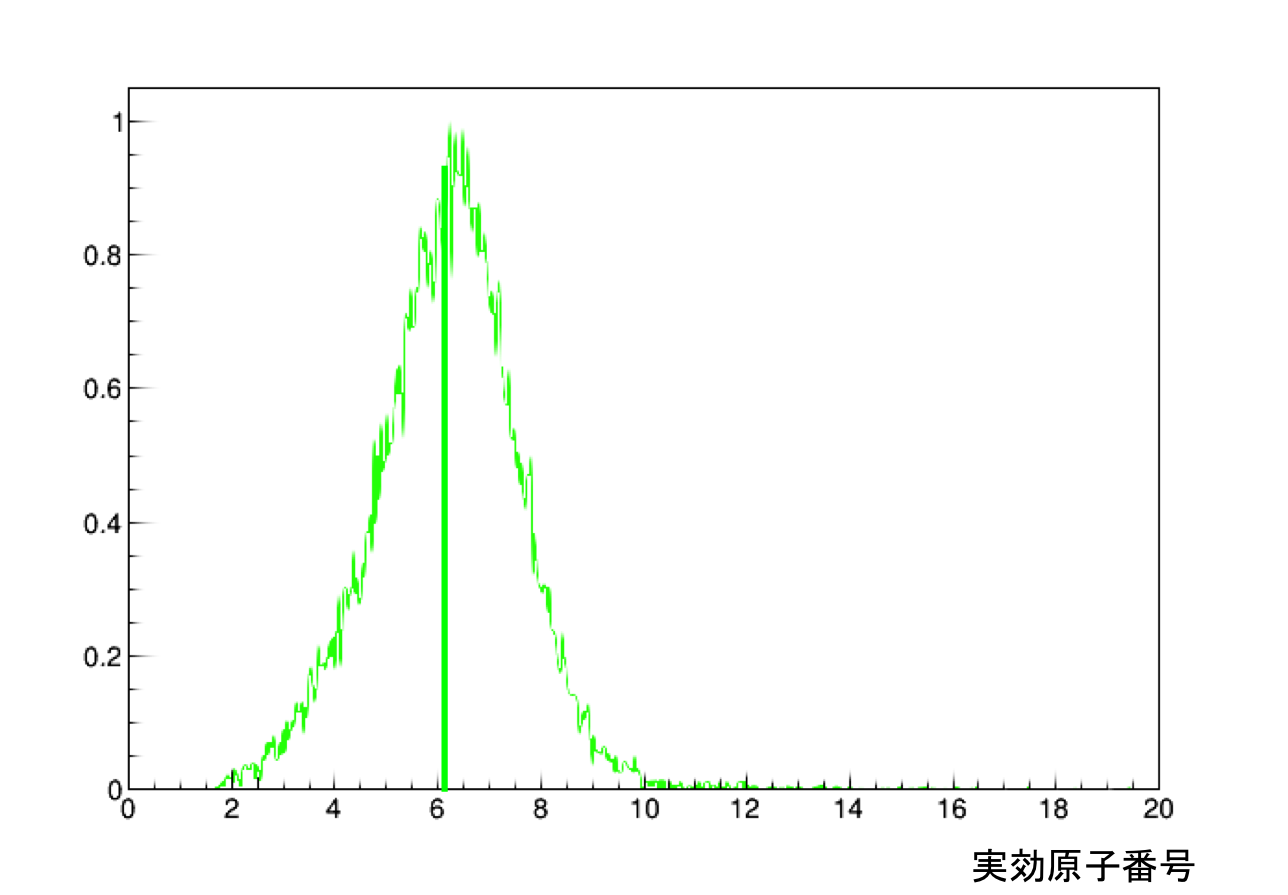
\includegraphics[bb=0.000000 0.000000 618.188896 429.564489,width=1.0\hsize]{image2/chapter5/Z_alcohol.png}
  \end{center}
\vspace{-1cm}
\caption*{アルコール}
 \end{minipage}
  \begin{minipage}{0.5\hsize}
  \begin{center}
   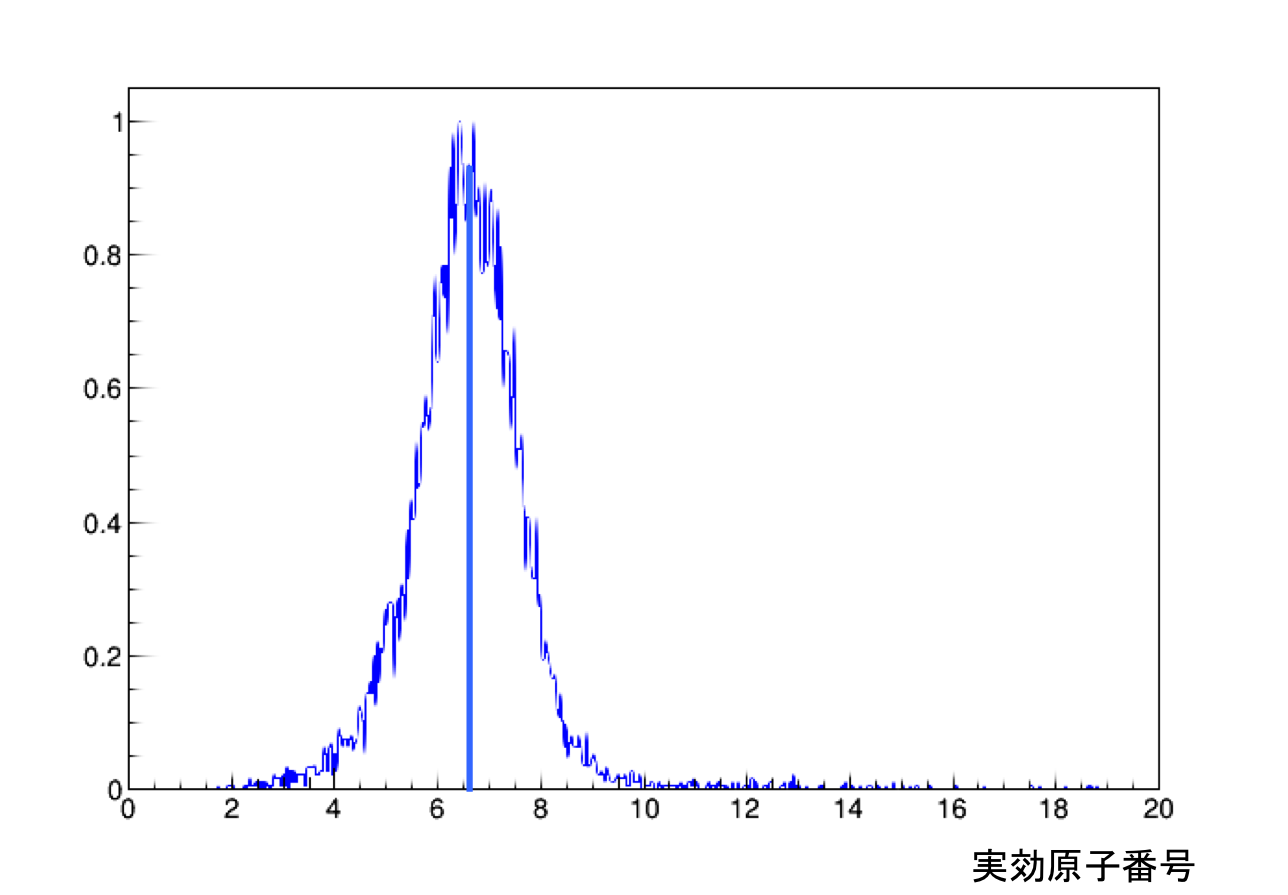
\includegraphics[bb=0.000000 0.000000 618.188896 429.564489,width=1.0\hsize]{image2/chapter5/Z_PMMA.png}
  \end{center}
\vspace{-1cm}
\caption*{PMMA}
 \end{minipage}
 \begin{center}
  \caption{それぞれのCT画像の原子番号同定結果}
  \label{fig:Z_identify}
  \end{center}
\end{figure}

% Table generated by Excel2LaTeX from sheet 'Sheet1'
\begin{table}[H]
  \centering
    \begin{tabular}{cccc}
    \toprule
          & 水     & アルコール & PMMA \\
    \midrule
    実効原子番号 & 7.42  & 6.16  &  \\
    実験値   & 7.83$\pm$1.02 & 6.28$\pm$1.23 & 6.59$\pm$0.885 \\
    \bottomrule
    \end{tabular}%
      \caption{それぞれの物質の実効原子番号と実験値}
  \label{tab:addlabel}%
\end{table}%


\section{K-edgeイメージング}

\subsection{ヨード造影剤の強調イメージング}

従来のエネルギー積分型の方式では実現できないイメージングがk 吸収端イメージングである。人体を構成する元素の大部分は原子番号が非常に小さいため,k 吸収端は低エネルギーレベルに存在するため,そのk 吸収端を捉えることは不可能であるが,造影剤として用いるガドリニウム(Gd) やヨード(I)のk 吸収端はそれぞれ50.2keV,33.2keV であり,k 吸収端の前後でデータの計測を行うことで造影剤の分布を特異的に示すことができる。例えばGd の場合bin0:40-49keV,bin1:50-59keV としそれぞれのbin でCT 画像を再構成した後,bin1 のCT 画像からbin0 のCT 画像を引き算することにより,造影剤を含んだ血管や組織などの明瞭な画像下が可能となる。
本稿では直径6cmのアクリル筒の中に水を満たし、ヨード造影剤(30mg/mL)を満たし、直径2cmのアクリル筒を入れた\Fref{fig:Iodine_phantom}を用いてヨード造影剤のK-edgeイメージングを管電圧120kV、管電流0.2mAで行った。

\begin{figure}[H]
 \begin{center}
 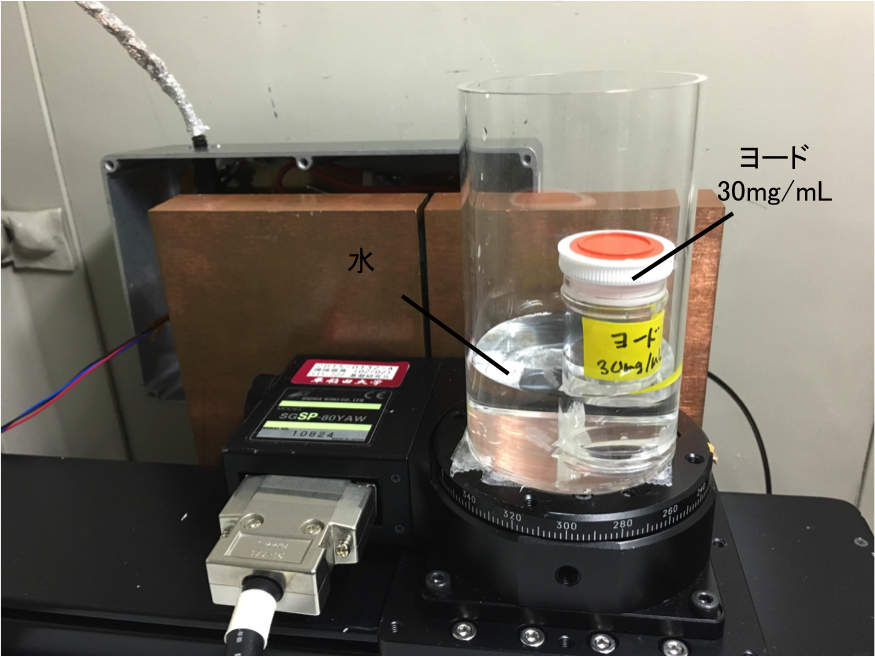
\includegraphics[bb=0.000000 0.000000 419.965283 315.333932,width=0.6\hsize]{image2/chapter5/Iodine_phantom.png} 
 \end{center}
 \caption{ヨードのK-edgeイメージングに用いたファントム}
 \label{fig:Iodine_phantom}
\end{figure}

ヨード造影剤(30mg/mL)の線減弱係数のエネルギー依存性は\Fref{fig:iodine_atten}のようになっている。この図に示すようにヨードのK吸収端は50.3keVであるが、実験的にK吸収端の位置を最初に確認した。


\begin{figure}[H]
 \begin{center}
 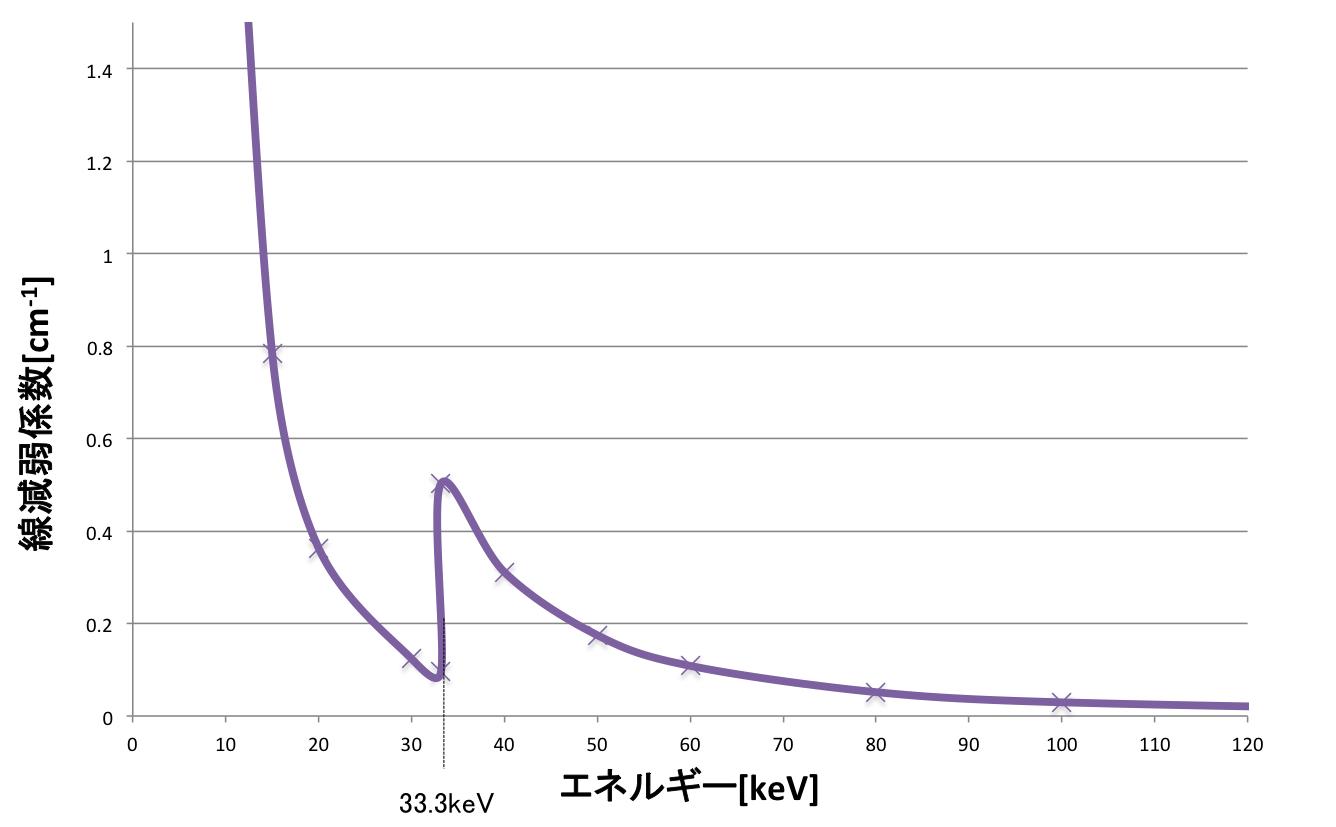
\includegraphics[bb=0.000000 0.000000 641.226992 396.927187,width=0.8\hsize]{image2/chapter5/iodine_atten.png} 
 \end{center}
 \caption{ヨード(30mg/mL)の線減弱係数のエネルギー依存性}
 \label{fig:iodine_atten}
\end{figure}


管電圧120kV、管電流0.2mAでMCA8000Dで100秒間取得したX線の全エネルギースペクトルを\Fref{fig:Iodine_spectrums}(左)に示す。
また同じ条件でヨードのK吸収端位置を確かめるためにヨード造影剤(140mg/mL)をMPPCの前に置いて取得したスペクトルを\Fref{fig:Iodine_spectrums}(右)に示す。

\begin{figure}[H]
 \begin{minipage}{0.5\hsize}
  \begin{center}
 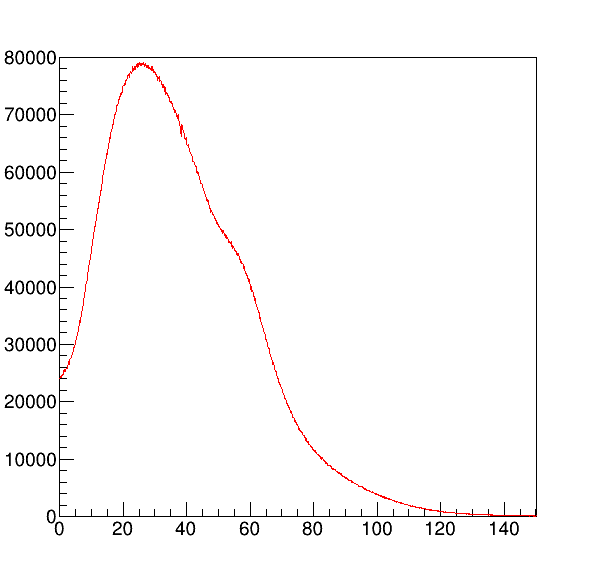
\includegraphics[bb=0.000000 0.000000 596.000000 574.000000,width=1\hsize]{image2/chapter5/all_energy.png} 
  \end{center}
 \end{minipage}
 \begin{minipage}{0.5\hsize}
  \begin{center}
 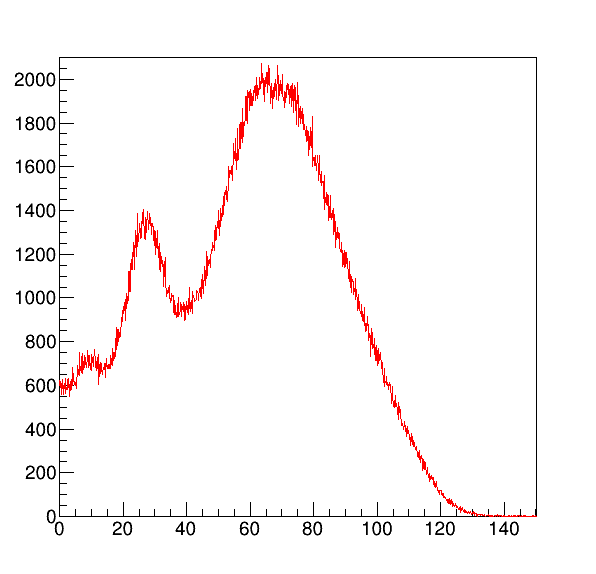
\includegraphics[bb=0.000000 0.000000 596.000000 574.000000,width=1\hsize]{image2/chapter5/I_kedge_100sec.png} 
  \end{center}
 \end{minipage}
 \begin{center}
  \caption{管電圧120kV、管電流0.2mAで測定したX線全エネルギースペクトル(左)とヨード造影剤140mg/mLをMPPCの前に置いて測定した時のスペクトル(右)}
  \label{fig:Iodine_spectrums}
  \end{center}
\end{figure}

スペクトルの窪んだ部分がヨードのK吸収端であり、この位置に閾値を設けて設定したX線スペクトルを\Fref{fig:over_I_kedge}に示す。\\

\begin{figure}[H]
 \begin{center}
 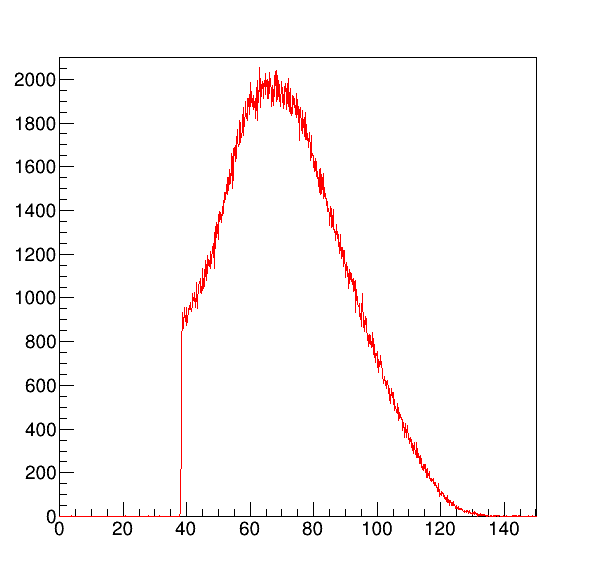
\includegraphics[bb=0.000000 0.000000 596.000000 574.000000,width=0.5\hsize]{image2/chapter5/over_I_kedge_100sec.png} 
 \end{center}
 \caption{ヨードのK吸収端に閾値を設けて測定したX線スペクトル}
 \label{fig:over_I_kedge}
\end{figure}

さらにK吸収端の±20keVにも閾値をdicriminatorで設定し、K吸収端の前20keVの帯域と後20keV帯域でそれぞれ投影データを取得し画像再構成を行った。

K吸収端の前20keVの帯域と後20keV帯域で取得したCT画像を\Fref{fig:Iodine_kedgeimage}に示す。

\begin{figure}[H]
 \begin{minipage}{0.5\hsize}
  \begin{center}
 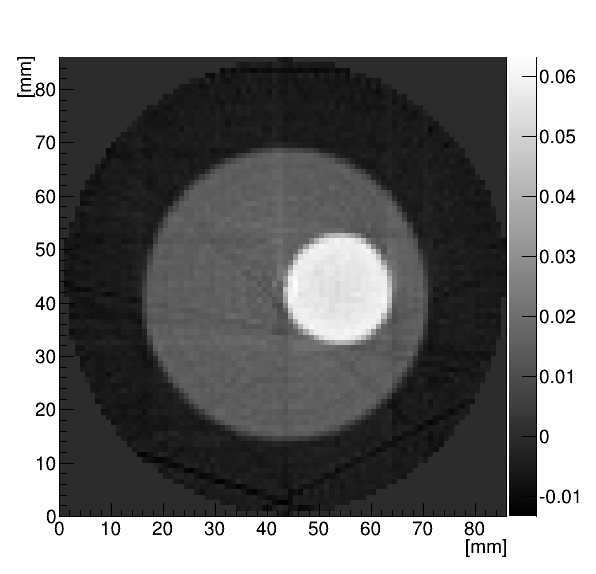
\includegraphics[bb=0.000000 0.000000 596.000000 574.000000,width=1\hsize]{image2/chapter5/image1_back.png} 
  \end{center}
 \end{minipage}
 \begin{minipage}{0.5\hsize}
  \begin{center}
 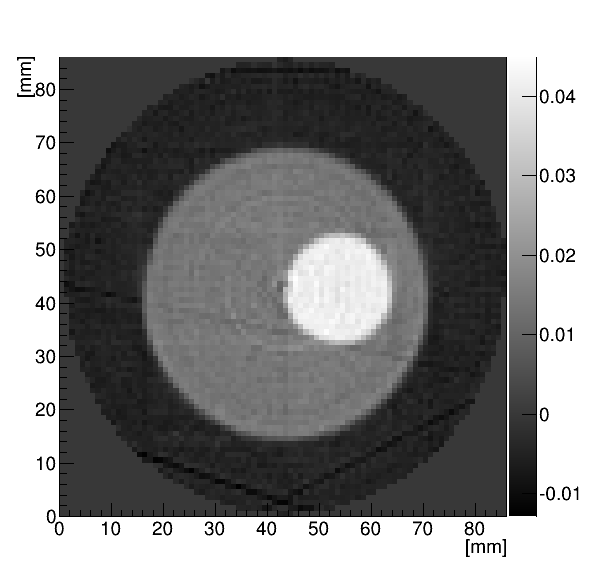
\includegraphics[bb=0.000000 0.000000 596.000000 574.000000,width=1\hsize]{image2/chapter5/image2_back.png} 
  \end{center}
 \end{minipage}
 \begin{center}
  \caption{ヨードのK-edgeの後20keV帯域で取得したCT画像(左)とK-edgeの前20keV帯域で取得したCT画像(右)}
  \label{fig:Iodine_kedgeimage}
  \end{center}
\end{figure}

ここで、ヨードのK-edgeの後20keV帯域で取得したCT画像を$\mu_+(x,y)$、ヨードのK-edgeの前20keV帯域で取得したCT画像を$\mu_-(x,y)$として、K-edgeイメージング$\mu_{\rm{k-edge}}(x,y)$、

\begin{align}
\mu_{\rm{k-edge}}(x,y)=\mu_+(x,y)- \mu_-(x,y)
\end{align}

を求めると\Fref{fig:subtraction}が得られる。

\begin{figure}[H]
 \begin{center}
 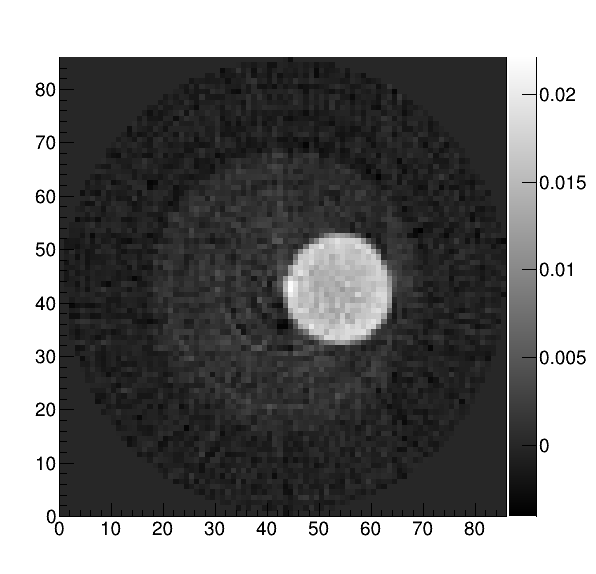
\includegraphics[bb=0.000000 0.000000 596.000000 574.000000,width=0.6\hsize]{image2/chapter5/image1-image2.png} 
 \end{center}
 \caption{K-edgeイメージング$\mu_{\rm{k-edge}}(x,y)$}
 \label{fig:subtraction}
\end{figure}

$\mu_+(x,y)$、$\mu_-(x,y)$、$\mu_{\rm{k-edge}}(x,y)$のヨード造影剤と水のコントラスト比を\Tref{tab:subtraction_contrast}に示す。

% Table generated by Excel2LaTeX from sheet 'Sheet1'
\begin{table}[htbp]
  \centering
    \begin{tabular}{cccc}
    \toprule
          & $\mu_+(x,y)$ & $\mu_-(x,y)$ & $\mu_{\rm{k-edge}}(x,y)$ \\
    \midrule
    Contrast ratio & \multirow{2}[2]{*}{2.4} & \multirow{2}[2]{*}{2.0} & \multirow{2}[2]{*}{3.9} \\
    ($\mu_I/\mu_w$) &       &       &  \\
    \bottomrule
    \end{tabular}%
     \caption{$\mu_+(x,y)$、$\mu_-(x,y)$、$\mu_{\rm{k-edge}}(x,y)$のコントラスト比の比較}
  \label{tab:subtraction_contrast}%
\end{table}%


\Tref{tab:subtraction_contrast}から明らかなように、$\mu_{\rm{k-edge}}(x,y)$におけるコントラスト比が他の2つの画像に比べて高いことがわかる。これはK-edge後の画像のCT値がヨードのみ高くなり、水はあまり変化しないため水のCT値は引き算によって相殺されるが、ヨードのCT値は差分が残るからである。これによって医療現場でのCT撮影時に血管ヨード造影剤用いた時に、血管のみのCT表示が可能となる。


\subsection{ヨード造影剤のがドリニウム造影剤のコントラスト反転}
K-edgeイメージングを用いることでK-edgeの位置が異なる二つの造影剤のコントラストを変化させる実験を行った。本実験ではヨード造影剤(30mg/mL)とがドリニウム造影剤(90mg/mL)を用いた。この二つの線減弱係数のエネルギー依存性を\Fref{fig:I_Gd_atten}に示す。


\begin{figure}[H]
 \begin{center}
 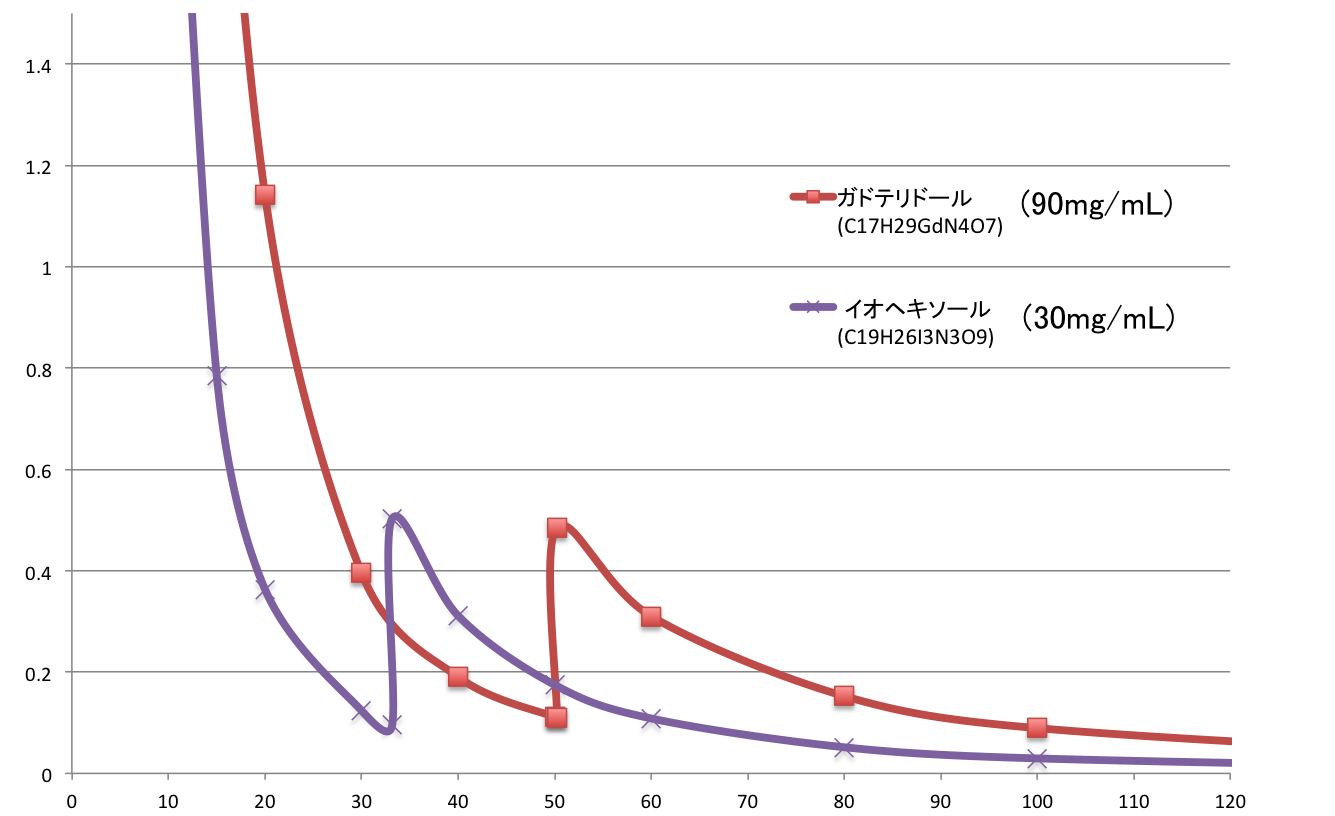
\includegraphics[bb=0.000000 0.000000 640.747032 391.647624,width=0.8\hsize]{image2/chapter5/I_Gd_atten.png} 
 \end{center}
 \caption{ヨード造影剤(30mg/mL)とガドリニム造影剤(90,g/mL)の線減弱係数のエネルギー依存性}
 \label{fig:I_Gd_atten}
\end{figure}

ヨードのK吸収端は33.3keV、ガドリニムのK吸収端は50.3keVである。本実験では\Tref{tab: vth2}のように閾値を定め、\Fref{fig:K-edge_window}のようなエネルギー帯域でそれぞれ投影データを取得し、CT画像を再構成した。

% Table generated by Excel2LaTeX from sheet 'Sheet1'
\begin{table}[htbp]
  \centering
    \begin{tabular}{ccccc}
    \toprule
    チャンネル & 1     & 2     & 3     & 4 \\
    \midrule
    閾値    & 30 keV & 50 keV & 70 keV  & 90 keV \\
    \bottomrule
    \end{tabular}%
      \caption{各チャンネルの閾値のエネルギー}
  \label{tab: vth2}%
\end{table}%

\begin{figure}[H]
 \begin{center}
 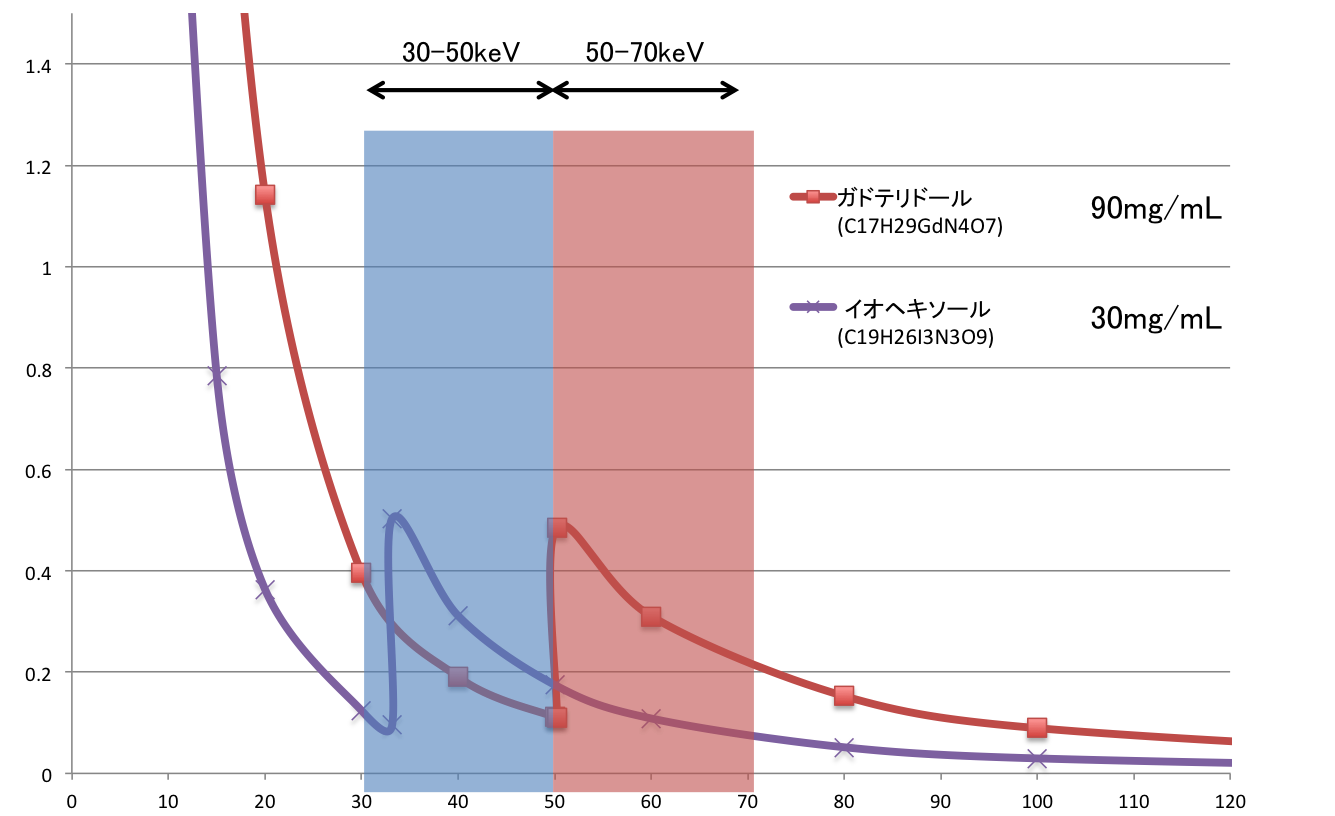
\includegraphics[bb=0.000000 0.000000 640.747032 391.647624,width=0.8\hsize]{image2/chapter5/K-edge_window.png} 
 \end{center}
 \caption{CT画像を取得するエネルギー帯域}
 \label{fig:K-edge_window}
\end{figure}


それぞれの閾値で管電圧120kV、管電流0.2mAで測定したX線のスペクトルを\Fref{fig:spectrum_hanten}に示す。



のようにような3つのエネルギーバンドそれぞれで投影データを作成し、CT画像を取得し画像にどのような変化が出るか検証した。それぞれのエネルギー帯域で得られた画像を\Fref{fig:hanten}に示す。

\begin{figure}[H]
 \begin{minipage}{0.5\hsize}
  \begin{center}
 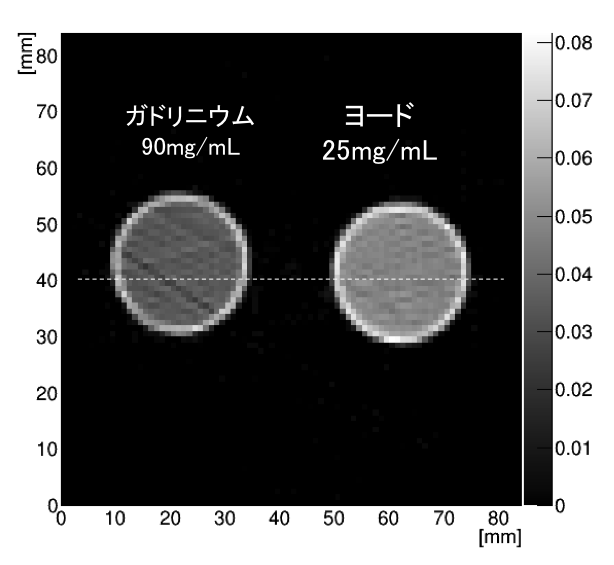
\includegraphics[bb=0.000000 0.000000 294.695638 271.177583,width=1\hsize]{image2/chapter5/hanten_30-50.png} 
  \end{center}
  \vspace{-1cm}
  \caption*{30-50keV}
 \end{minipage}
 \begin{minipage}{0.5\hsize}
  \begin{center}
 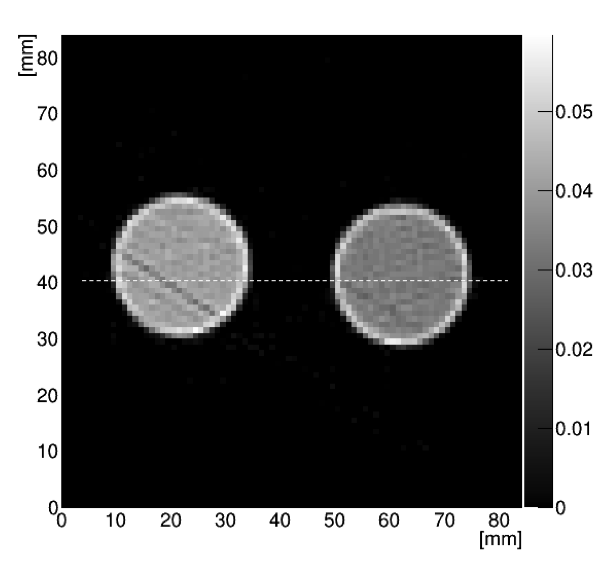
\includegraphics[bb=0.000000 0.000000 294.695638 272.137503,width=1\hsize]{image2/chapter5/hanten_50-70.png} 
  \end{center}
    \vspace{-1cm}
  \caption*{50-70keV}
 \end{minipage}
  \begin{minipage}{0.5\hsize}
     \hspace{3.5cm}
 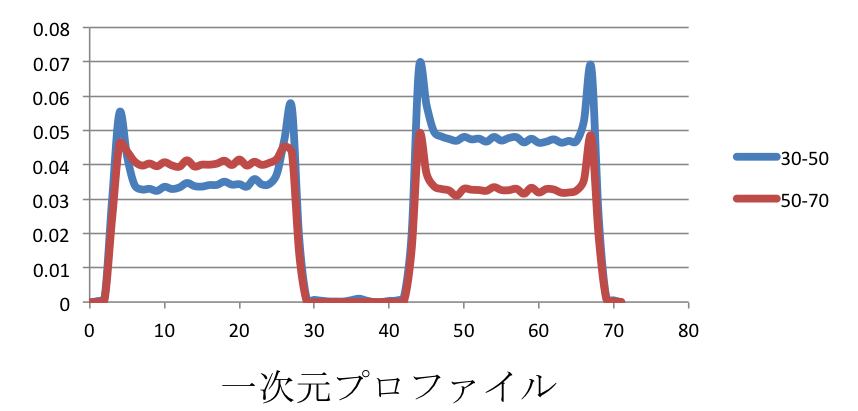
\includegraphics[bb=0.000000 0.000000 411.805957 197.263693,width=1.4\hsize]{image2/chapter5/hanten_profile.png} 
 \end{minipage}
 \begin{center}
  \caption{30-50keVと50-70keVの二つのエネルギー帯域で取得したガドリニウム造影剤とヨード造影剤のCT画像とその一次元プロファイル}
  \label{fig:hanten}
  \end{center}
\end{figure}

\Fref{fig:hanten}を見ると30-50keVのエネルギーバンドではヨードの方がCT値が高いが、50-70keVにおいてはガドリニウムの方がヨードよりCT値が高くなっている。これは\Fref{fig:I_Gd_atten}に示したように、K吸収端を境に線減弱係数の大小が反転し30-50keVにおいてはヨードの方が線減弱係数が高く、50-70keVにおいてはガドリニウムの方が線減弱係数が高くなったからである。






